This chapter is dedicated to the exposition and analysis of our experimental results. We shall commence by showcasing the performance of our model and meticulously comparing it against the baseline model derived from preceding work. The comparison will span two crucial stages - the generation of weak labels and the ultimate segmentation performance.

Beyond the comparative assessment, we thrust into statistical validation using the t-test. This step solidifies our evidence by testing the hypothesis concerning the improvement observed in our results.

Through this dual approach, with a comparative study augmented by rigorous statistical validation, we aim to furnish a comprehensive demonstration of the capabilities and advancements of our model over existing methods. We perform separate ablation studies to delve into the effect of potential key components on the segmentation performance. Collectively, these analyses form the backbone of our arguments, underpinning the significant contribution of our work in advancing state-of-the-art segmentation tasks.

\section{Weak Label generation}

A crucial component of our training pipeline is the process of weak label generation. This stage, marked by utilising centerline coordinates for creating a preliminary weak mask and subsequent enhancement through training with limited fully-connected data, plays a pivotal role in determining the final segmentation model performance.

With an emphasis on the decisive influence of the quality of weak labels, we present an in-depth comparison of the performance of our approach against the baseline model (Table \ref{tab:mask-generation-comparison}). The results are examined in terms of the Dice Similarity Coefficient (DSC), with the details presented using the format \(\mu_i \pm \sigma_{i}\), where \(\mu\) and \(\sigma\) denote the mean and variance of the DSC on test instances respectively.

\begin{table}[ht]
    \begin{subtable}[b]{\textwidth}
        \centering
        \begin{tabular}{c | c | c}
        Model & Average DSC (Axial) & Average DSC (Coronal) \\
        \hline
        Baseline & \(0.5553 \pm 0.0755\)  & \(0.5463 \pm 0.0986\)\\
        \hline
        Our Method & \(\mathbf{0.8084 \pm 0.0695}\) & \(\mathbf{0.6941 \pm 0.0871}\) 
       \end{tabular}
       \caption{Average Case Comparison}
       \label{tab:average-mask-generation}
    \end{subtable}
    \vfill
    \begin{subtable}[b]{\textwidth}
        \centering
        \begin{tabular}{c | c | c}
        Model & Best DSC (Axial) & Best DSC (Coronal) \\
        \hline
        Baseline & 0.6305 & 0.6559\\
        \hline
        Our Method & \(\mathbf{0.8843}\) & \(\mathbf{0.8251}\)
       \end{tabular}
       \caption{Best Case Comparison}
       \label{tab:best-mask-generation}
    \end{subtable}
     \caption{Weak Label Generation Comparison}
     \label{tab:mask-generation-comparison}
\end{table}

In both the average and best-case scenarios, our method exhibits an appreciable edge over the baseline in terms of DSC values for axial and coronal images as shown in Tables \ref{tab:average-mask-generation} and \ref{tab:best-mask-generation}. It is noteworthy to highlight that our approach significantly outperforms the baseline derived from preceding work \cite{Ali2022}. In terms of average performance, we observe uplifts of 45.58\% and 27.05\% for Axial T2 and Coronal images, respectively.

The sizable improvement is also evident when examining the best performance for each case type. With a remarkable increase of 40.24\% for Axial T2 and a substantial 25.8\% rise for Coronal T2 images, our approach convincingly demonstrates its effectiveness.

These results underline the efficacy of our method in generating high-quality weak labels that substantially enhance the final segmentation performance. These findings offer a promising perspective on the potential of our strategy to contribute meaningfully to advancements in terminal ileum segmentation tasks.

\subsection{Visual Validation of Model Performance}
We offer a graphical representation of our model's performance in Figure \ref{fig:comparison-mask-gt}, providing a direct comparison between the generated weak masks and the corresponding ground truth annotations across both Coronal and Axial modalities.

Upon detailed observation, one can notice that the weak masks generated by our model align significantly well with the ground truth, as evidenced by the regions coloured yellow, which represent either the ground truth segmentation or the generated mask.

As portrayed in the paired images (Figs. \ref{fig:gt-axial} and \ref{fig:mask-axial} for Axial T2; Figs. \ref{fig:gt-coronal} and \ref{fig:mask-coronal} for Coronal T2), the substantial overlaps between our generated mask and the ground truth are noteworthy, with hardly discernible discrepancies.

This visual illustration accentuates the robustness of our model in generating highly accurate weak masks, thereby closely mirroring the ground truth. Consequently, our model demonstrates remarkable potential in facilitating precise and dependable terminal ileum segmentation tasks, bridging the gap between machine-generated weak masks and human-annotated ground truths.

\begin{figure}[htp]
    \centering
    \begin{subfigure}[b]{0.48\textwidth}
        \centering
        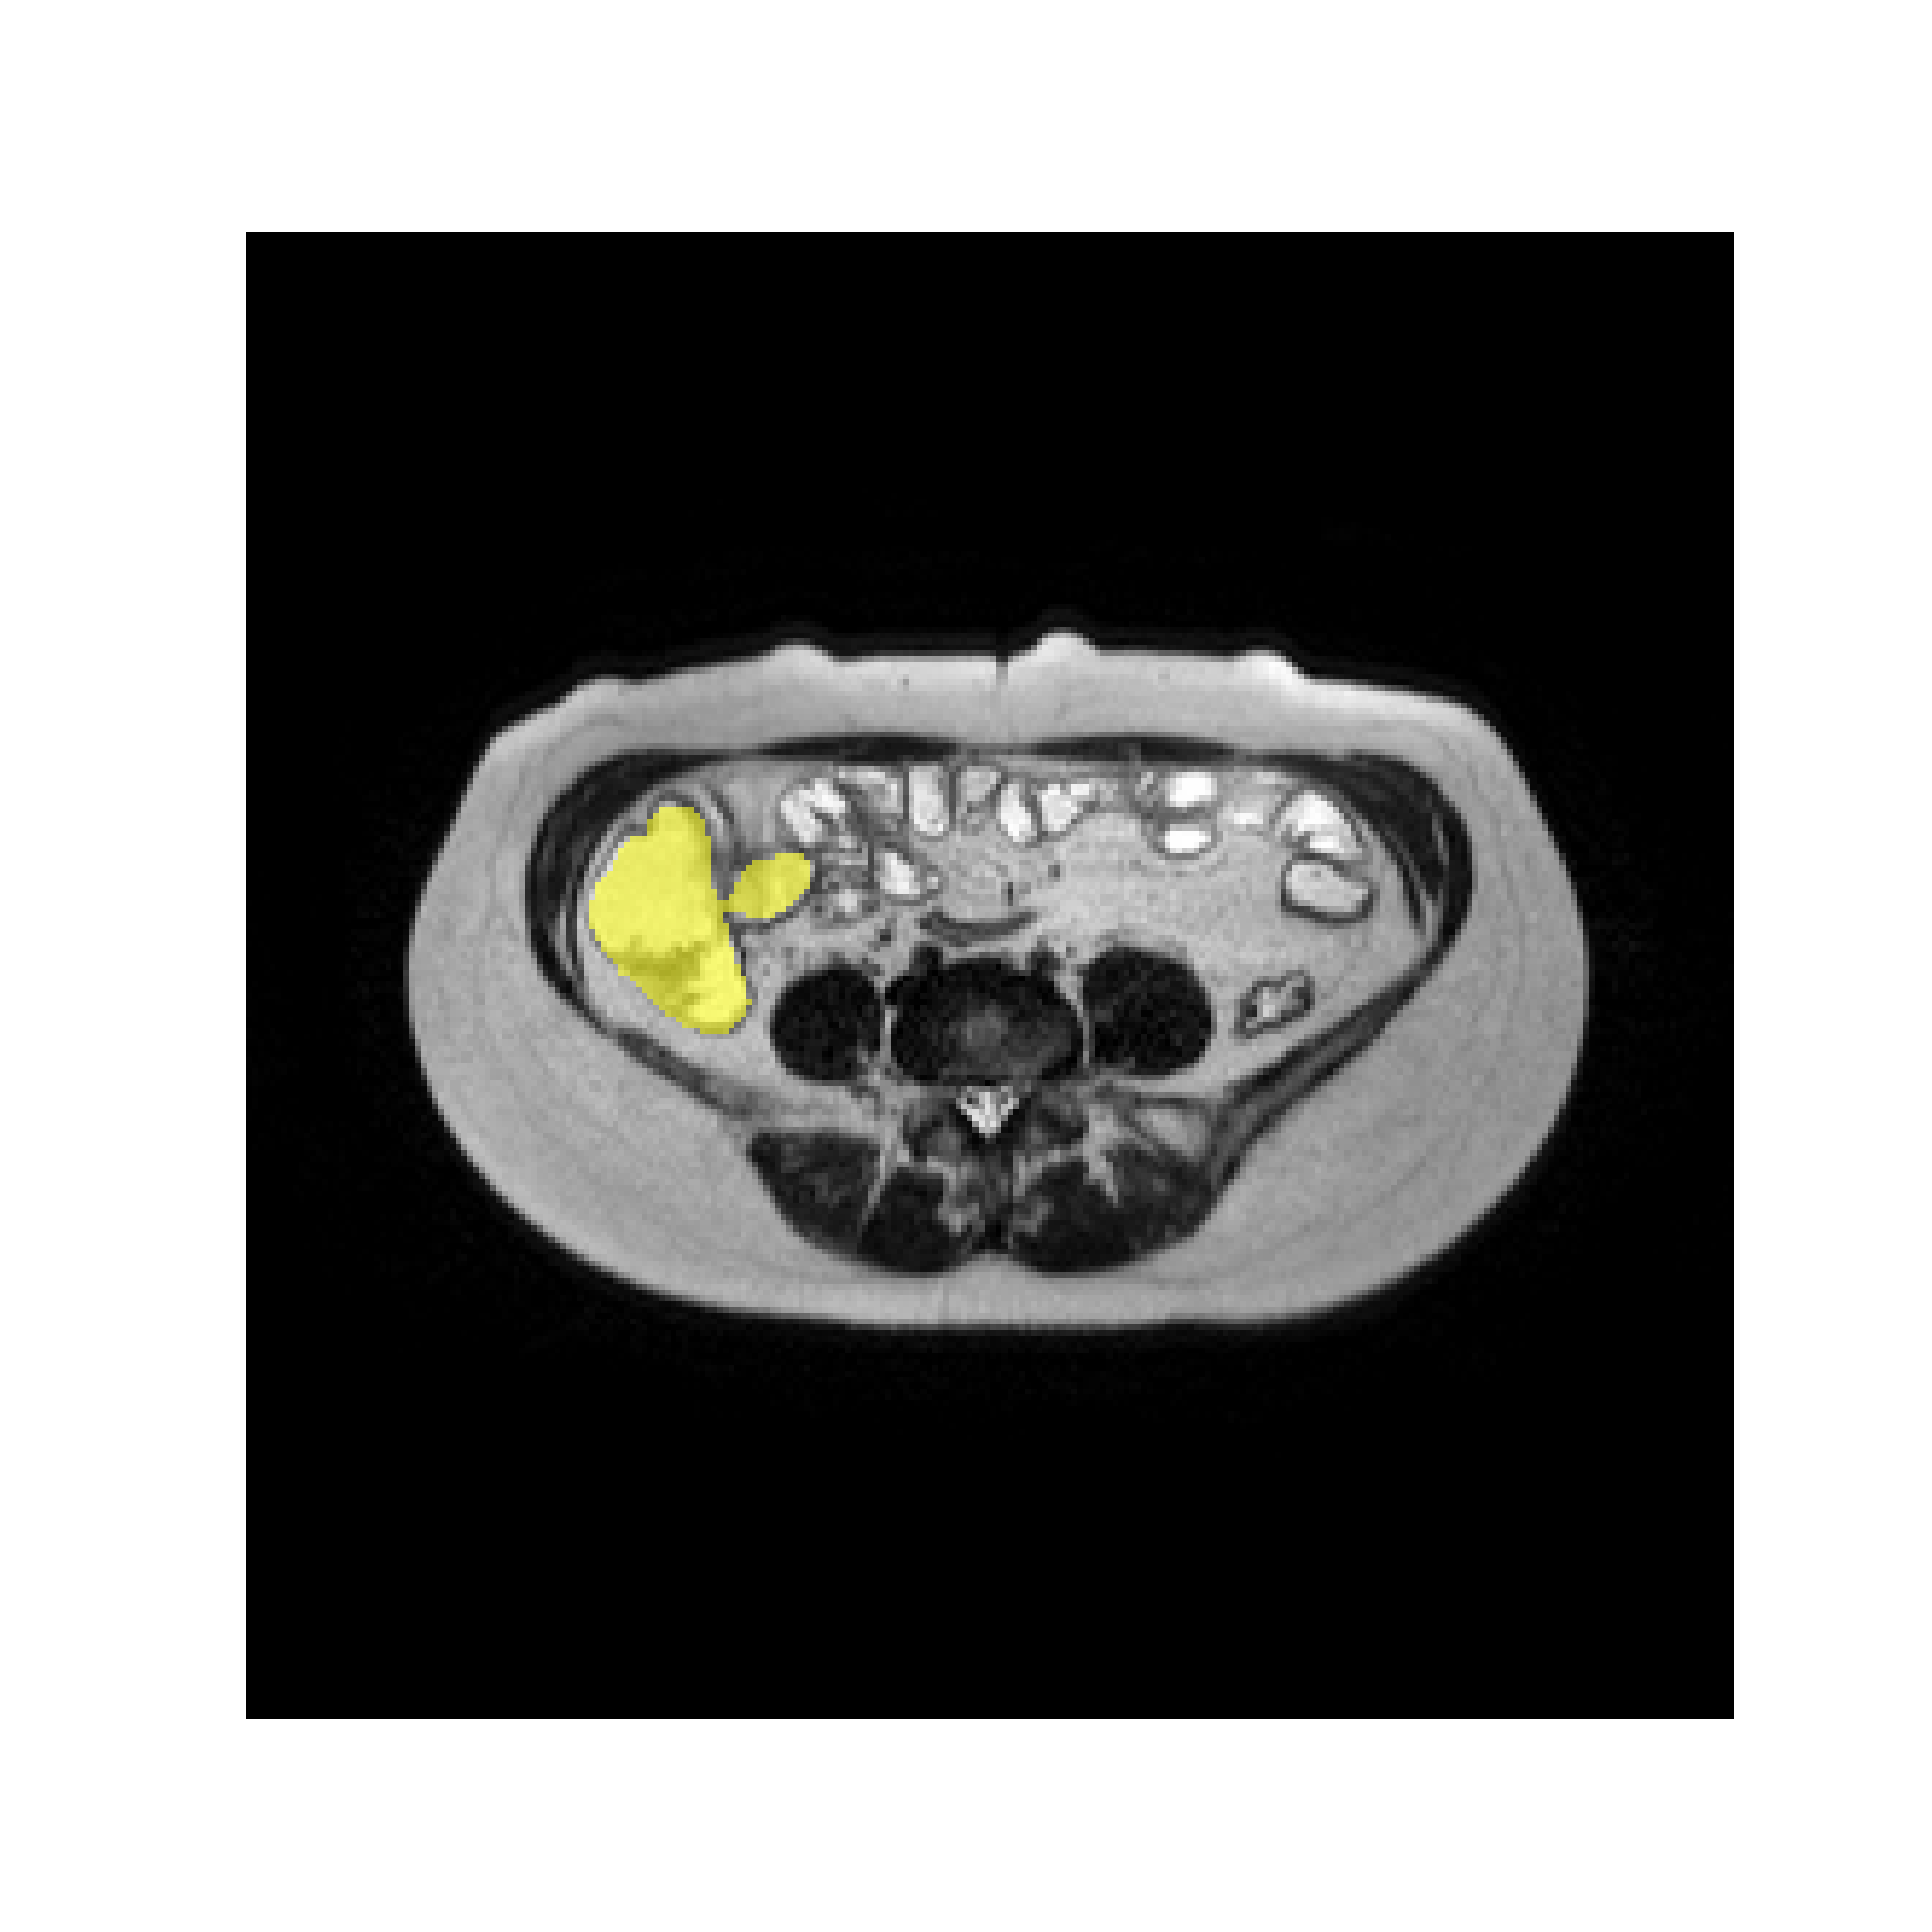
\includegraphics[width=\textwidth]{./figures/weak_mask_axial_gt.png}
        \caption{Ground Truth on Axial T2}
        \label{fig:gt-axial}
    \end{subfigure}
    \hfill
    \begin{subfigure}[b]{0.48\textwidth}
        \centering
        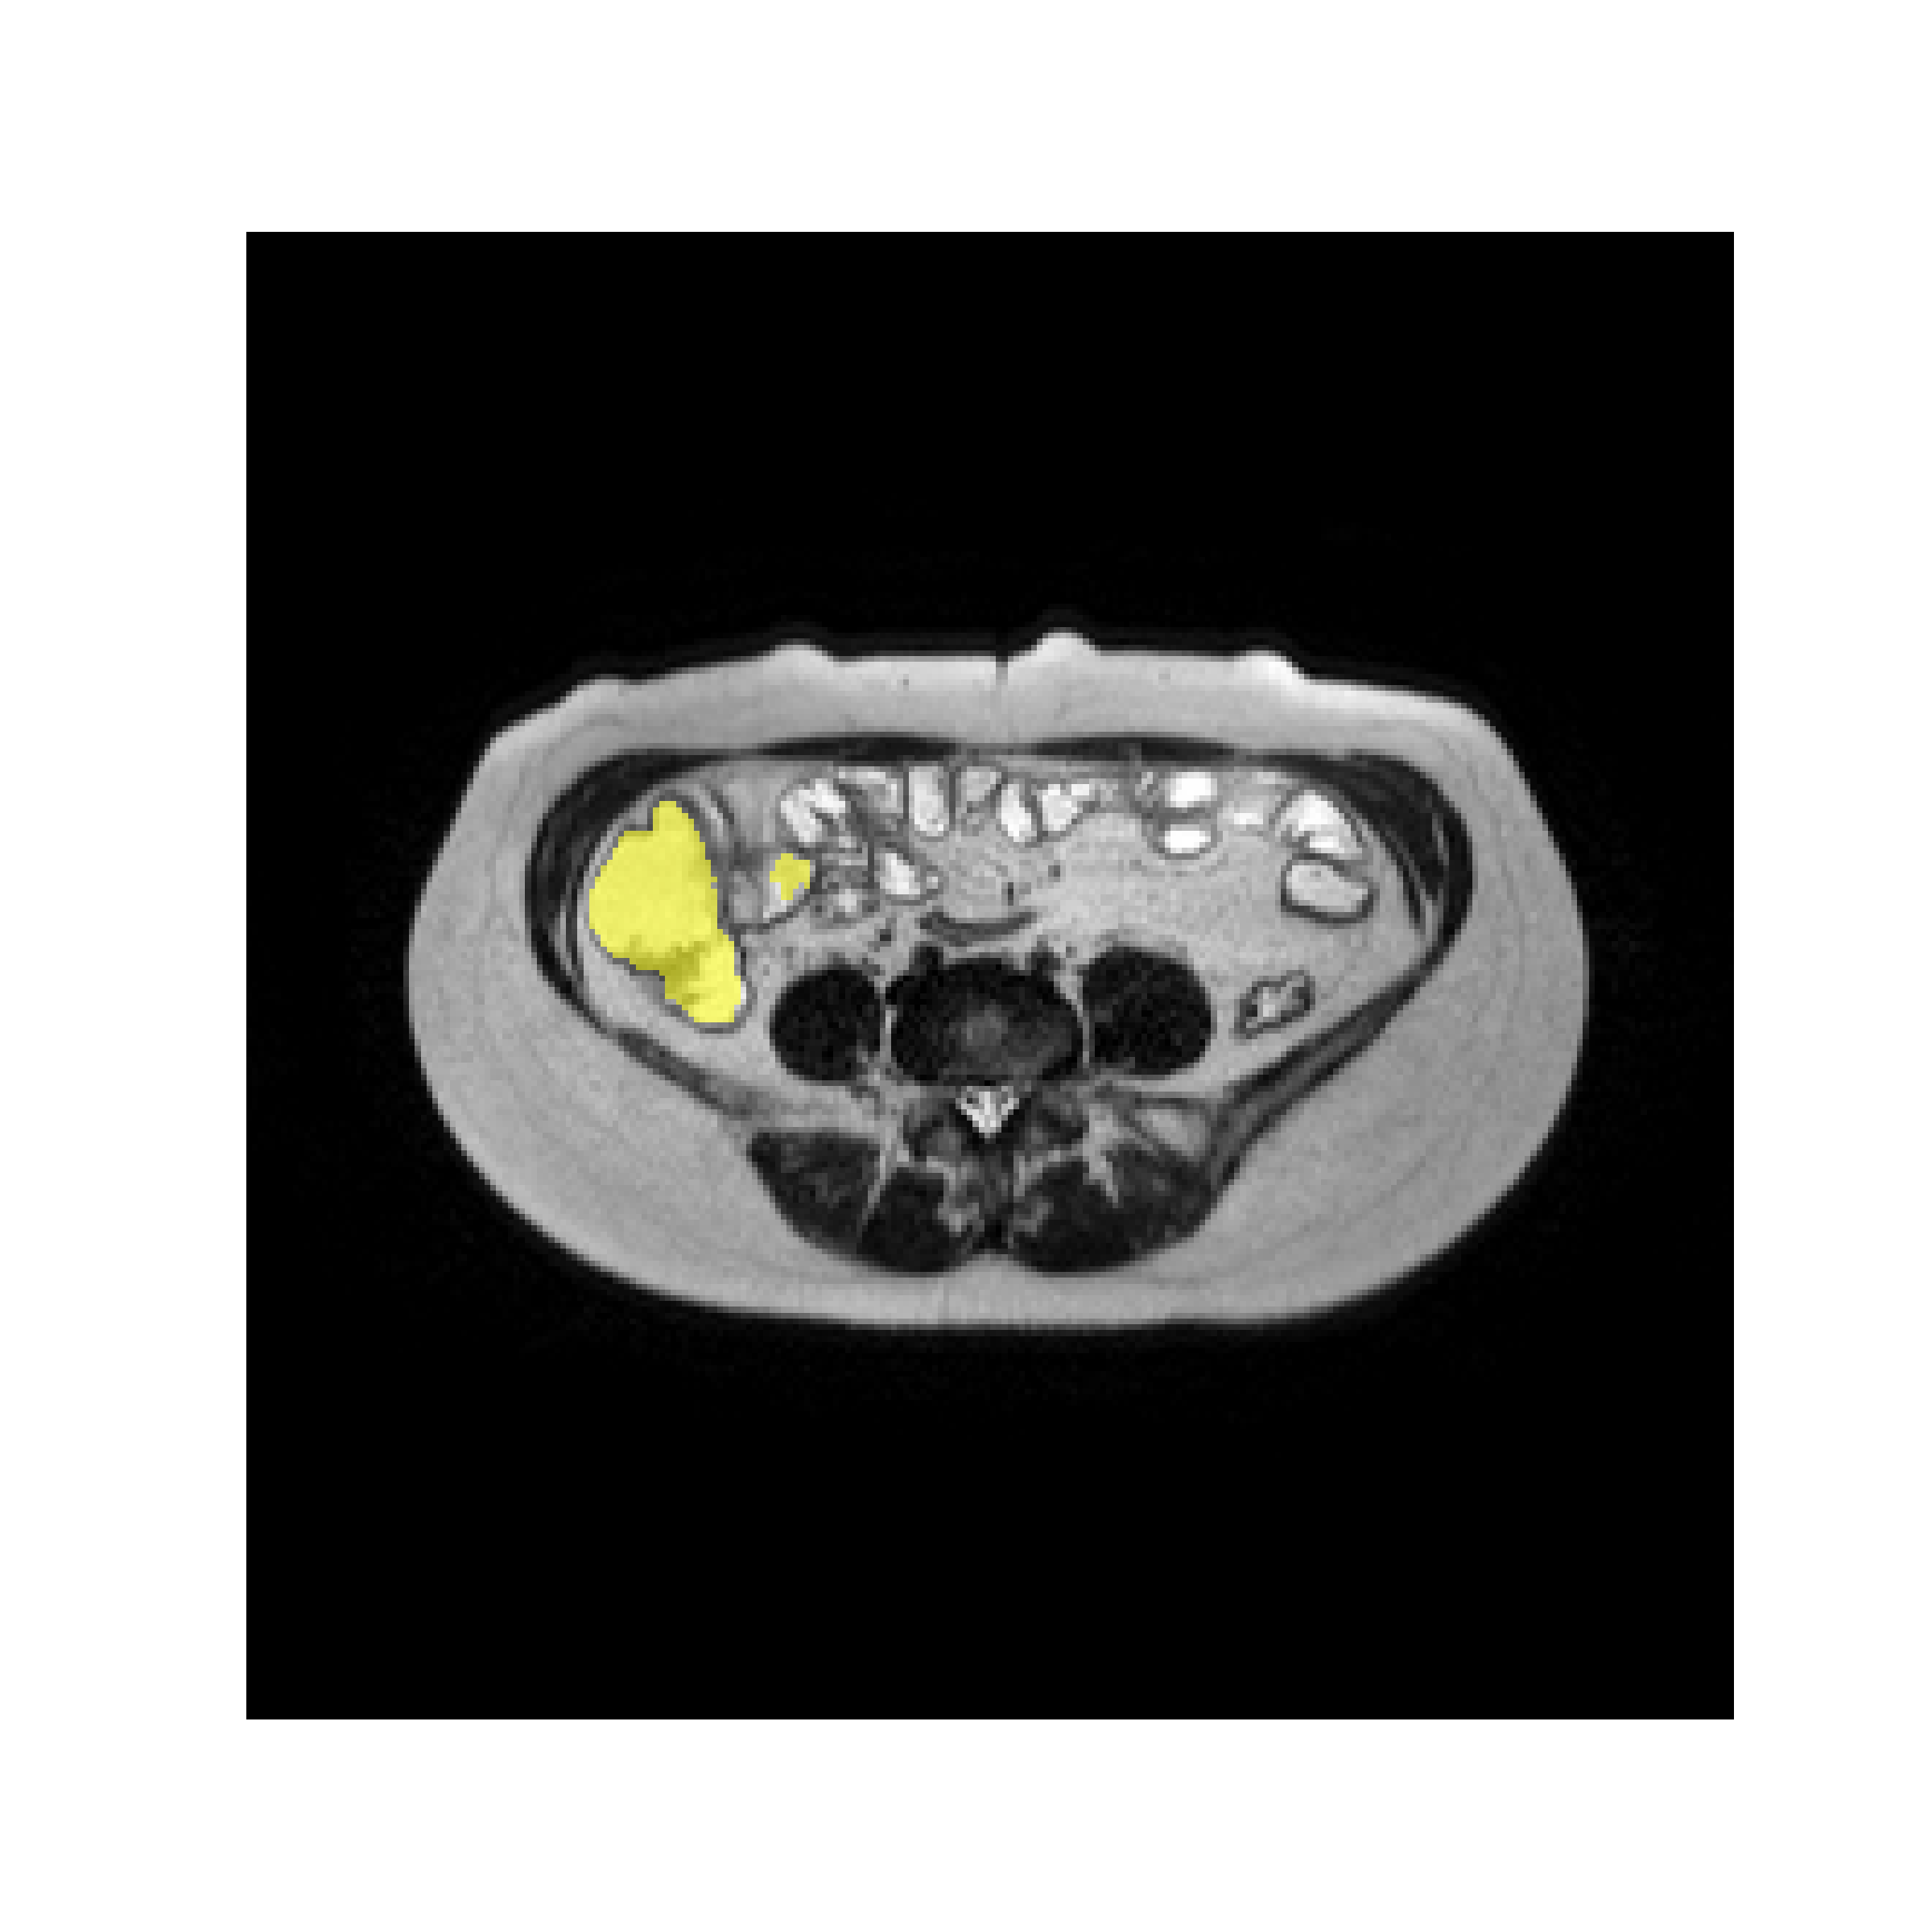
\includegraphics[width=\textwidth]{./figures/weak_mask_axial_medsam.png}
        \caption{Weak Mask on Axial T2}
        \label{fig:mask-axial}
    \end{subfigure}
    \vskip\baselineskip
    \begin{subfigure}[b]{0.48\textwidth}
        \centering
        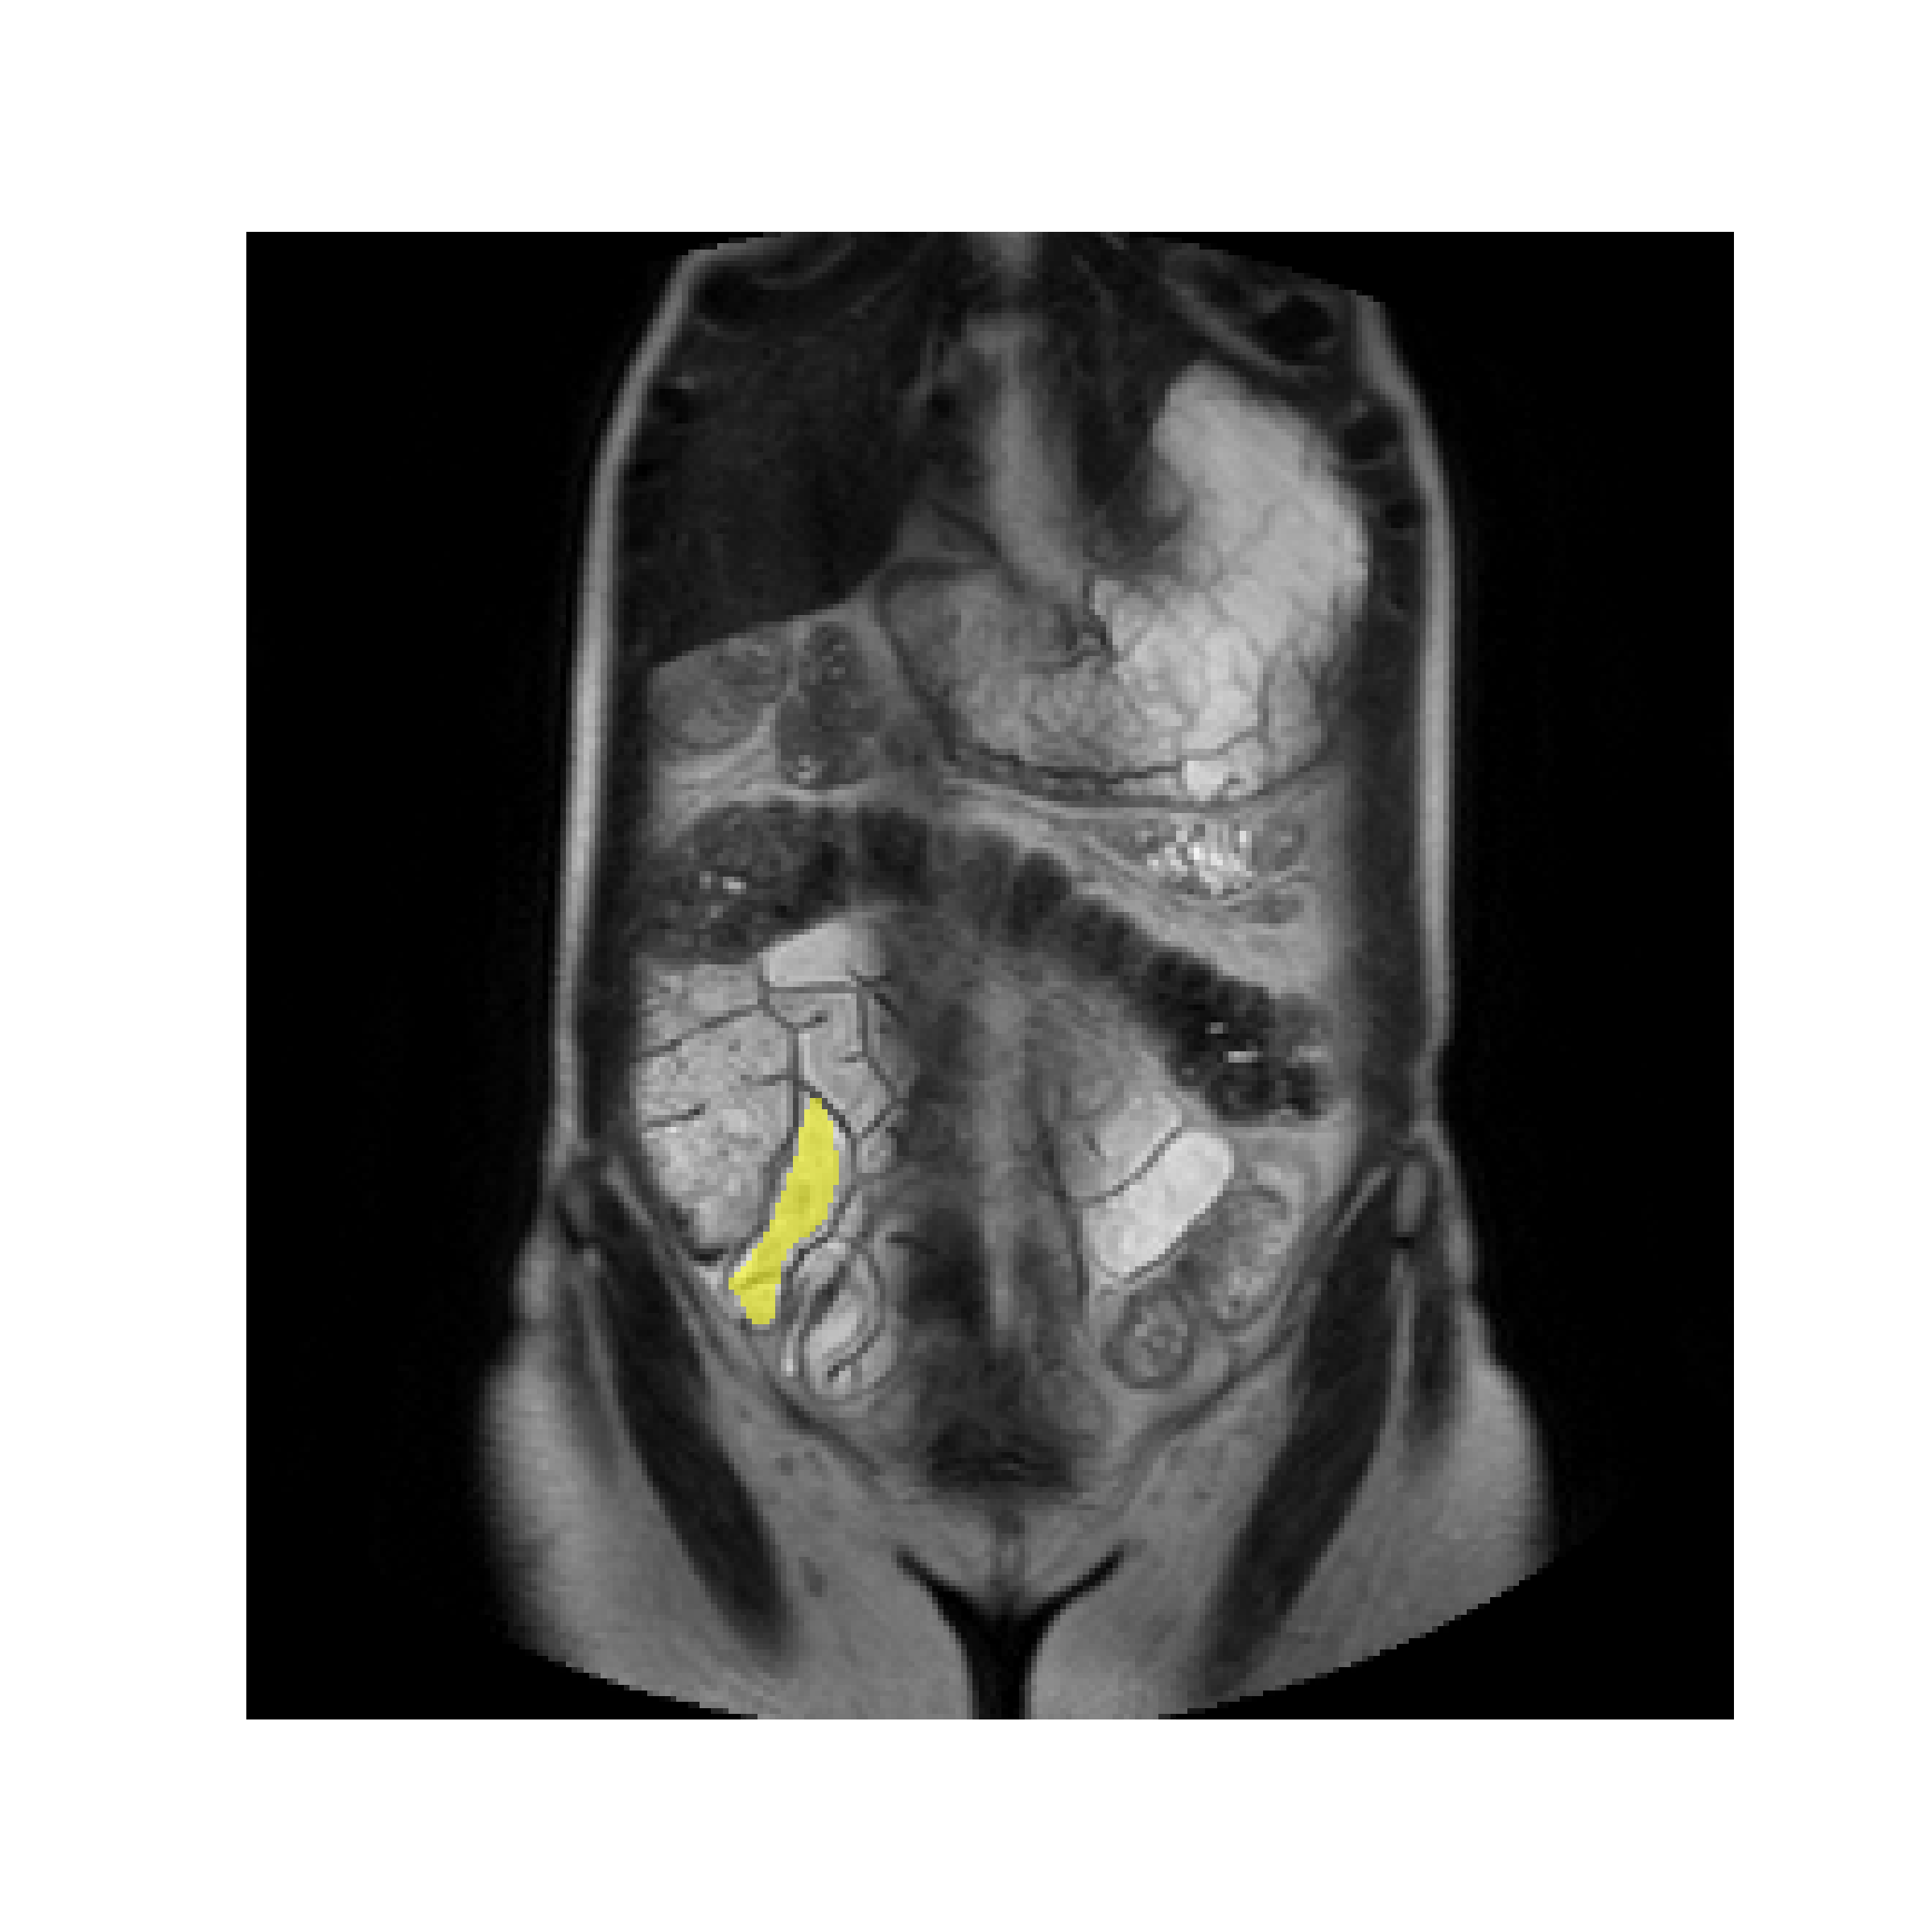
\includegraphics[width=\textwidth]{./figures/weak_mask_coronal_gt.png}
        \caption{Ground Truth on Coronal T2}
        \label{fig:gt-coronal}
    \end{subfigure}
    \hfill
    \begin{subfigure}[b]{0.48\textwidth}
        \centering
        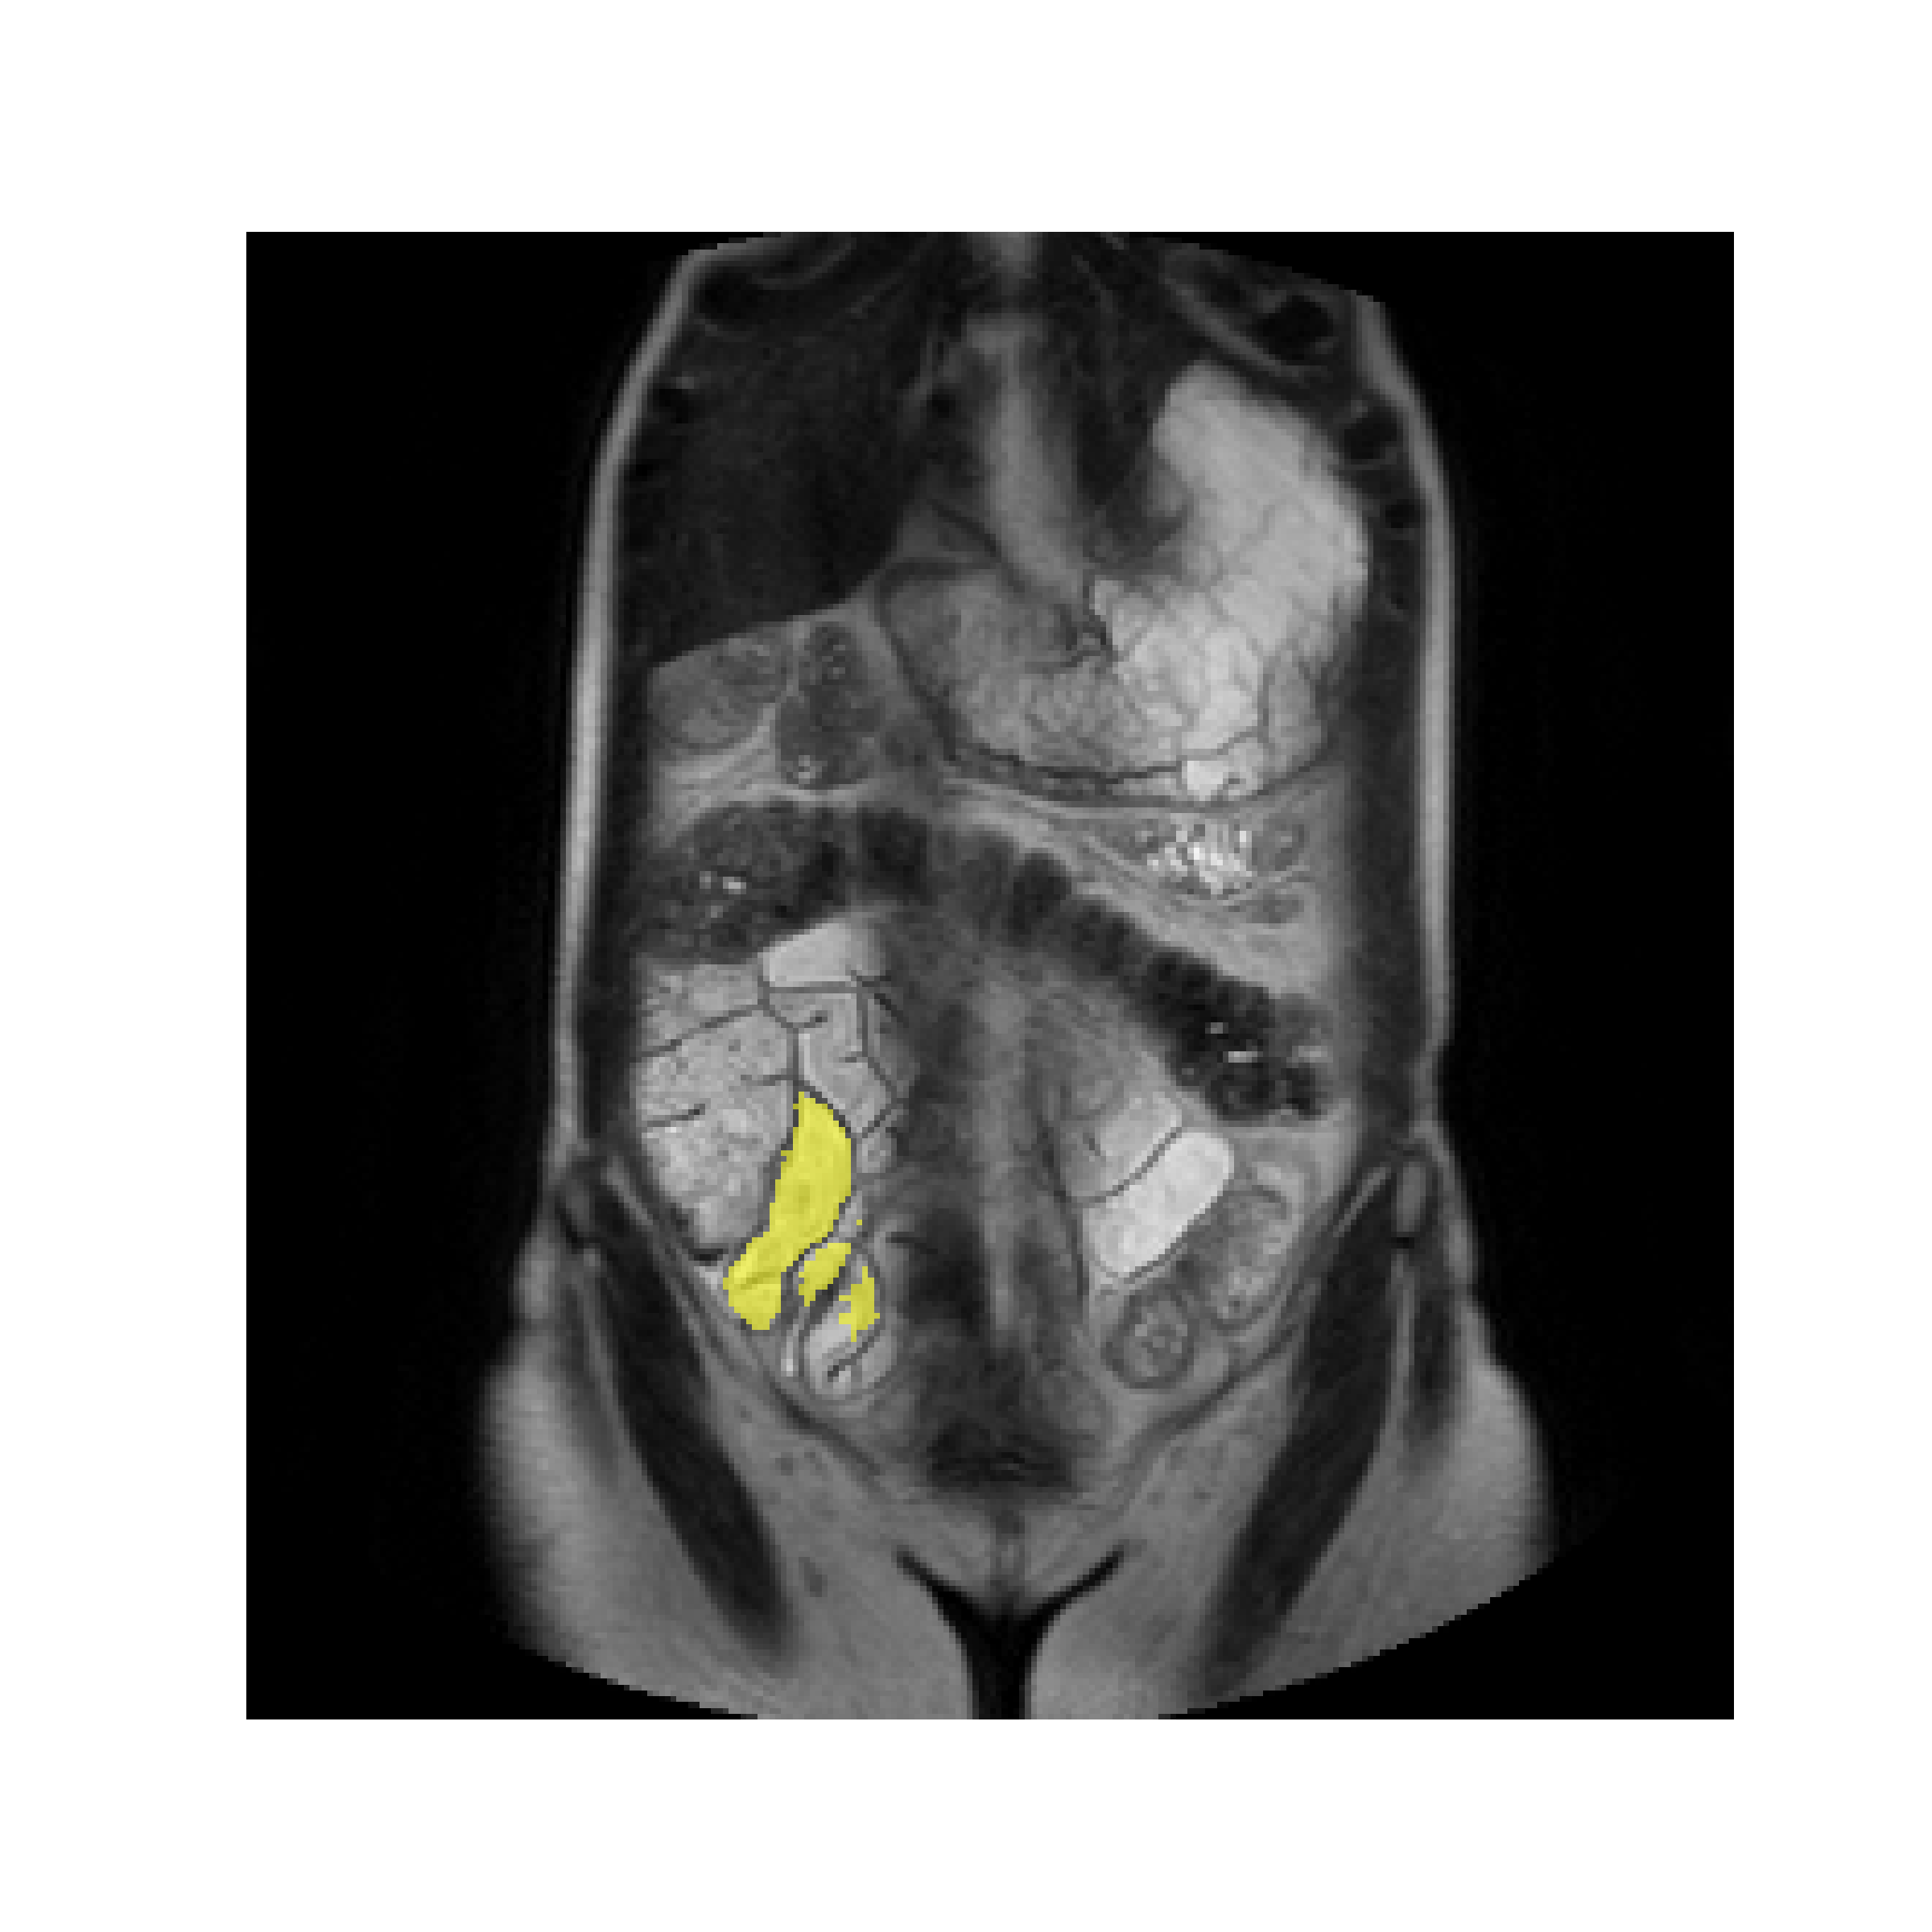
\includegraphics[width=\textwidth]{./figures/weak_mask_coronal_medsam.png}
        \caption{Weak Mask on Coronal T2}
        \label{fig:mask-coronal}
    \end{subfigure}
       \caption{A Cross-Model Comparison between Ground Truth and Generated Weak Masks}
       \label{fig:comparison-mask-gt}
\end{figure}
\subsection{Statistical Evaluation for Establishing Significance}

In a bid to confirm the statistical significance of the enhancements realized through our approach, we employed the two-tailed t-test. Setting a significance level of 0.05, we sought a comparative study across modalities between the baseline and the outcomes generated through our technique.

It is important to note that the t-test utilized is an independent two-sample t-test as it takes into consideration results gathered separately from two distinct groups: the baseline results and those generated by our approach.

The table below presents a detailed view of the t-test outcomes:

\begin{table}[ht]
\centering
\begin{tabular}{c|c|c|c}
Modality & \(t\) statistic & \(p\) value & significance level \\
\hline
Axial & 3.9138 & 0.0029 & 0.05 \\
\hline
Coronal & 2.525 & 0.0355 & 0.05
\end{tabular}
\end{table}

These test results stand out because both cases' \(p\) values fall below the set significance level. This provides compelling evidence to dismiss our null hypothesis, confirming significant improvements in our weak label generation. Consequently, we can assertively state that our approach tangibly enhances the performances of the processes under study.

\section{T.I. Segmentation}
Completing our sophisticated two-phase training, we embarked on an evaluation phase for both the baseline and our model. The test set comprised 7 and 9 out of 38 and 48 human annotations for axial and coronal cases. The metrics employed for this evaluation were in line with the previously discussed Dice Similarity Coefficient (DSC), and the evaluation results are showcased in Table \ref{tab:seg}. 
\begin{table}[ht]
    \begin{subtable}[b]{\textwidth}
        \centering
        \begin{tabular}{c | c | c}
        Model & Average DSC (Axial) & Average DSC (Coronal) \\
        \hline
        Baseline & \(0.5691 \pm 0.1759\)  & \(0.5824 \pm 0.1195\)\\
        \hline
        Our Method & \(\mathbf{0.7372 \pm 0.1692}\) & \(\mathbf{0.6724 \pm 0.1174}\) 
       \end{tabular}
       \caption{Average Case Comparison}
       \label{tab:average-seg}
    \end{subtable}
    \vfill
    \begin{subtable}[b]{\textwidth}
        \centering
        \begin{tabular}{c | c | c}
        Model & Best DSC (Axial) & Best DSC (Coronal) \\
        \hline
        Baseline & 0.6573 & 0.6711\\
        \hline
        Our Method & \(\mathbf{0.8975}\) & \(\mathbf{0.8023}\)
       \end{tabular}
       \caption{Best Case Comparison}
       \label{tab:best-seg}
    \end{subtable}
     \caption{Weak Label Generation Comparison}
     \label{tab:seg}
\end{table}

A comprehensive analysis of the results reveals that our method significantly outperforms the baseline regarding DSC values for both axial and coronal images. As Tables \ref{tab:average-seg} and \ref{tab:best-seg} portray, our model exhibits marked superiority over the baseline derived from prior work in routine and best-case performance scenarios.

Specifically, for average performance, our model delivers a robust improvement of 29.54\% and 15.45\% for Axial and Coronal T2 images, respectively. Such substantial enhancements are also mirrored in optimal performance scenarios, reaping an impressive 36.54\% and 19.55\% increase for Axial and Coronal cases.

These rewarding outcomes vividly exemplify the substantial progression achieved over previous methodologies in terms of segmentation performance, reinforcing our commitment to continuously refine and improve our approaches in confronting the challenges posed by Crohn's disease.
\subsection{Visual Validation of Model Performance}
To illustrate the performance disparity between the baseline methodology and our refined approach, we provide a side-by-side visual comparison. This graphical representation (\autoref{fig:comparison-pred}) focuses on Axial T2 images, showcasing predictions generated by both the baseline model and our technique in contrast with the ground truth.

\begin{figure}[htp]
\centering
\begin{subfigure}[b]{0.47\textwidth}
\centering
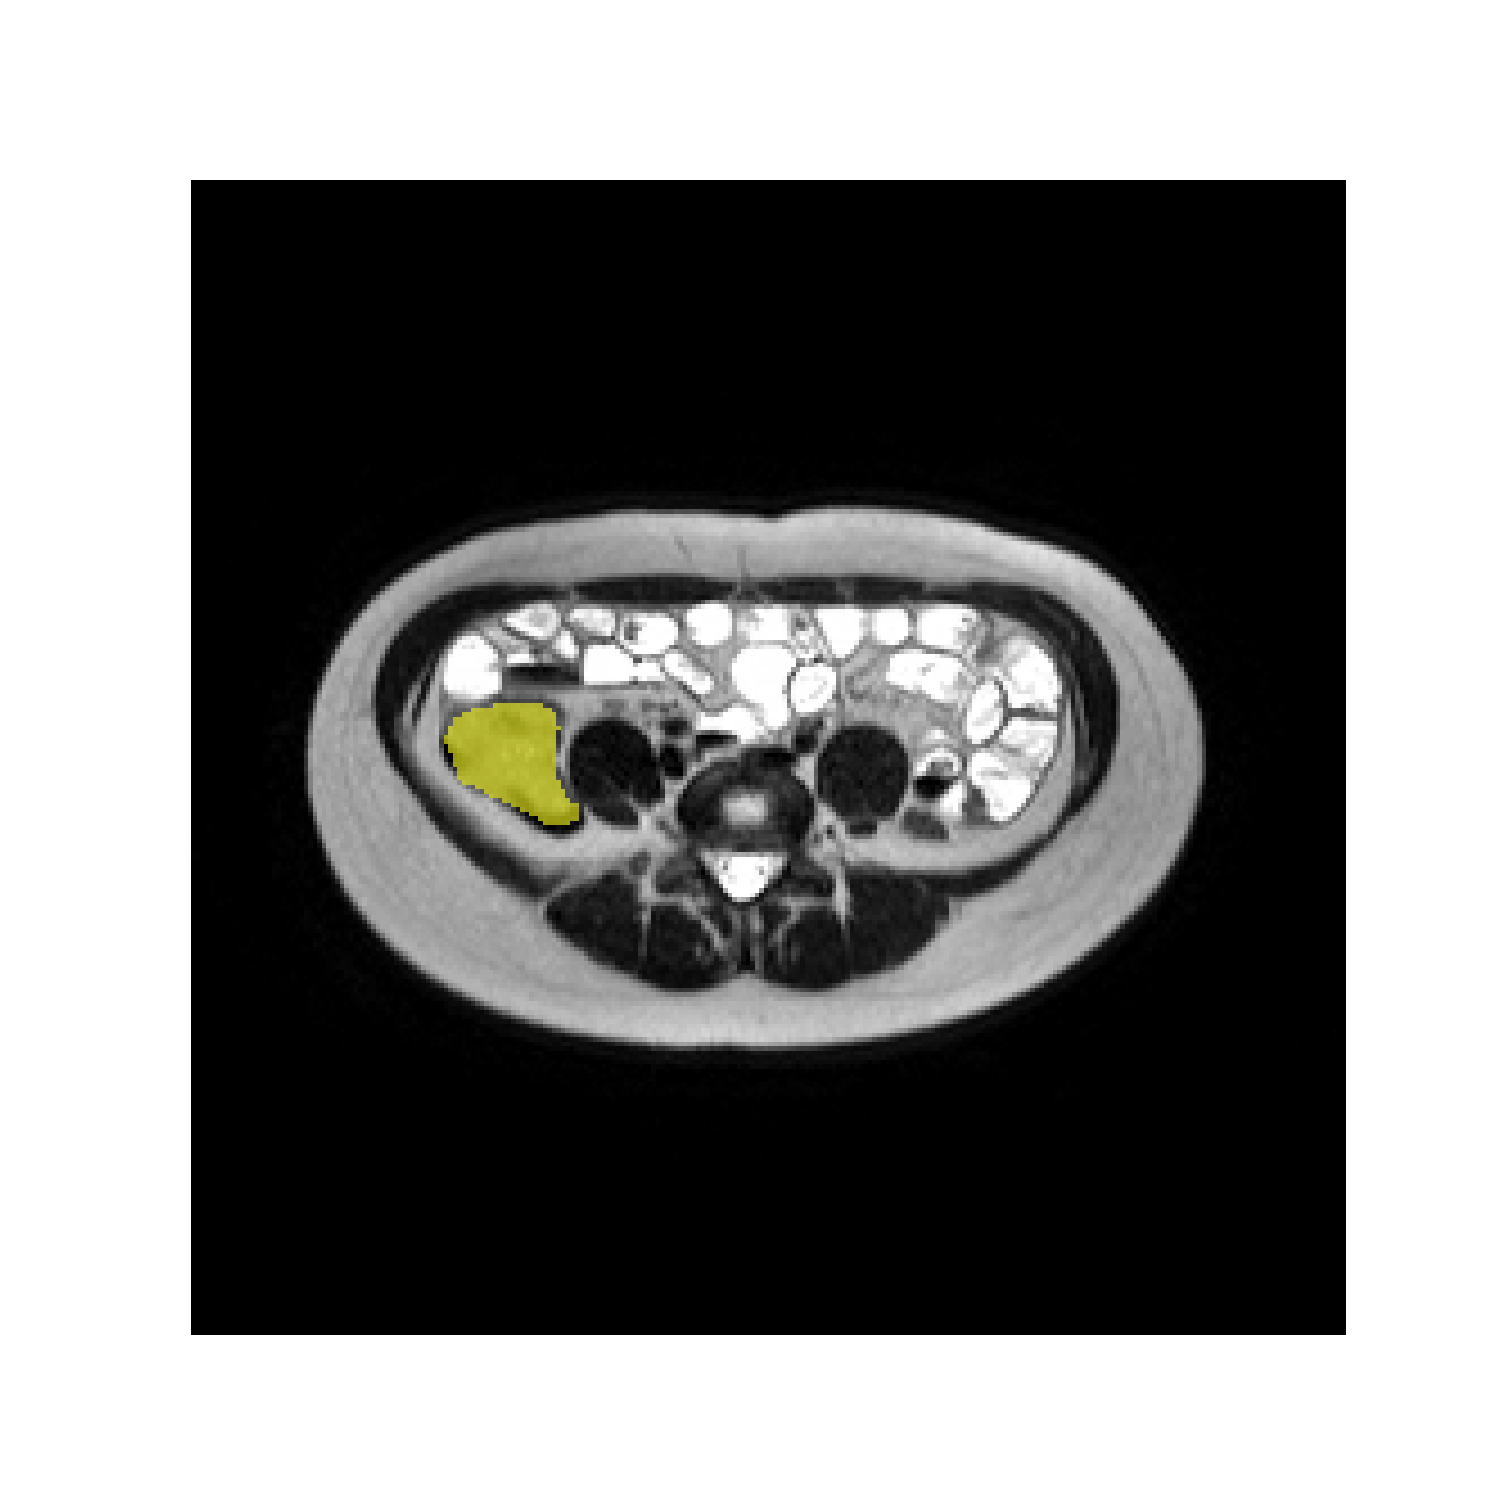
\includegraphics[width=\textwidth]{./figures/seg_gt.png}
\caption{Ground Truth}
\label{fig:gt}
\end{subfigure}
\hfill
\begin{subfigure}[b]{0.47\textwidth}
\centering
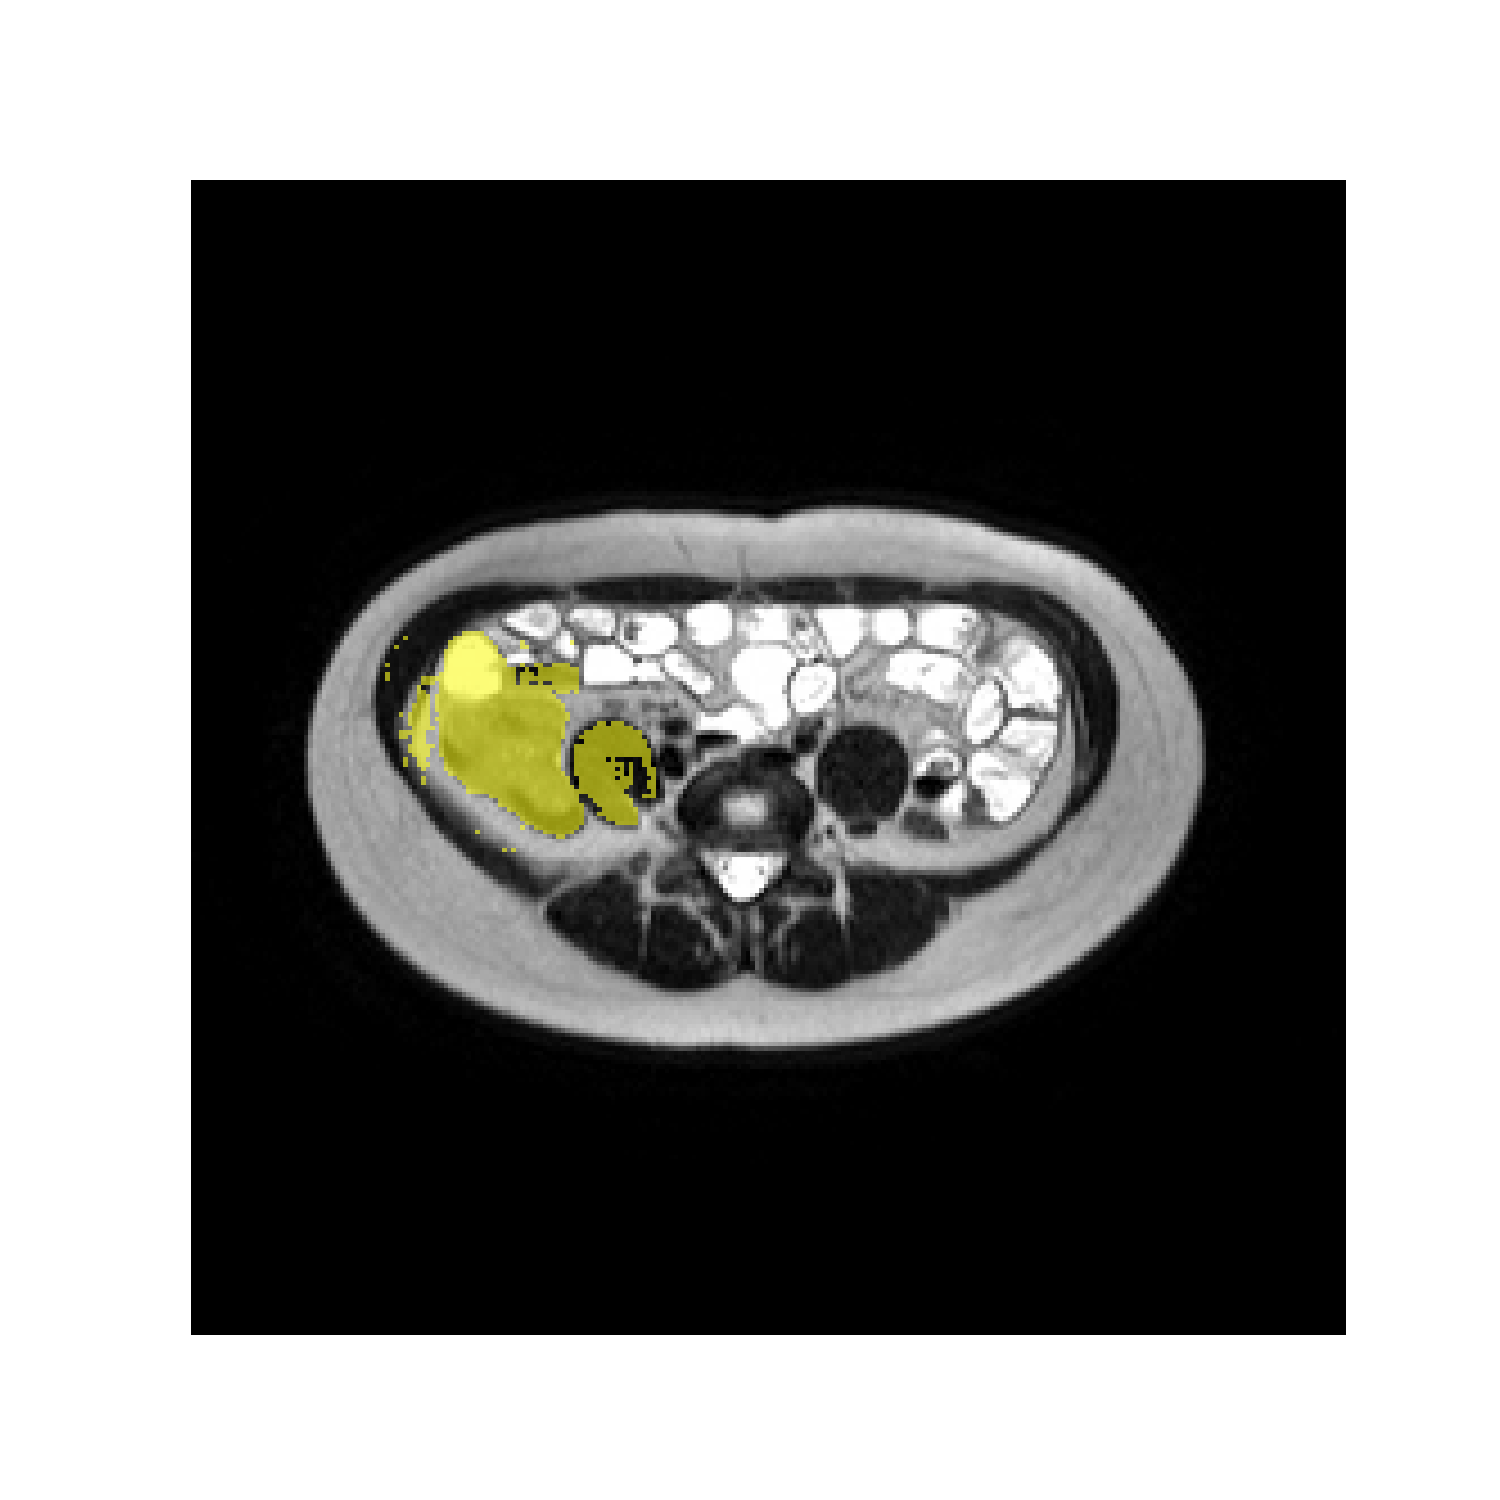
\includegraphics[width=\textwidth]{./figures/seg_baseline.png}
\caption{Baseline Prediction}
\label{fig:baseline-pred}
\end{subfigure}
\hfill
\begin{subfigure}[b]{0.47\textwidth}
\centering
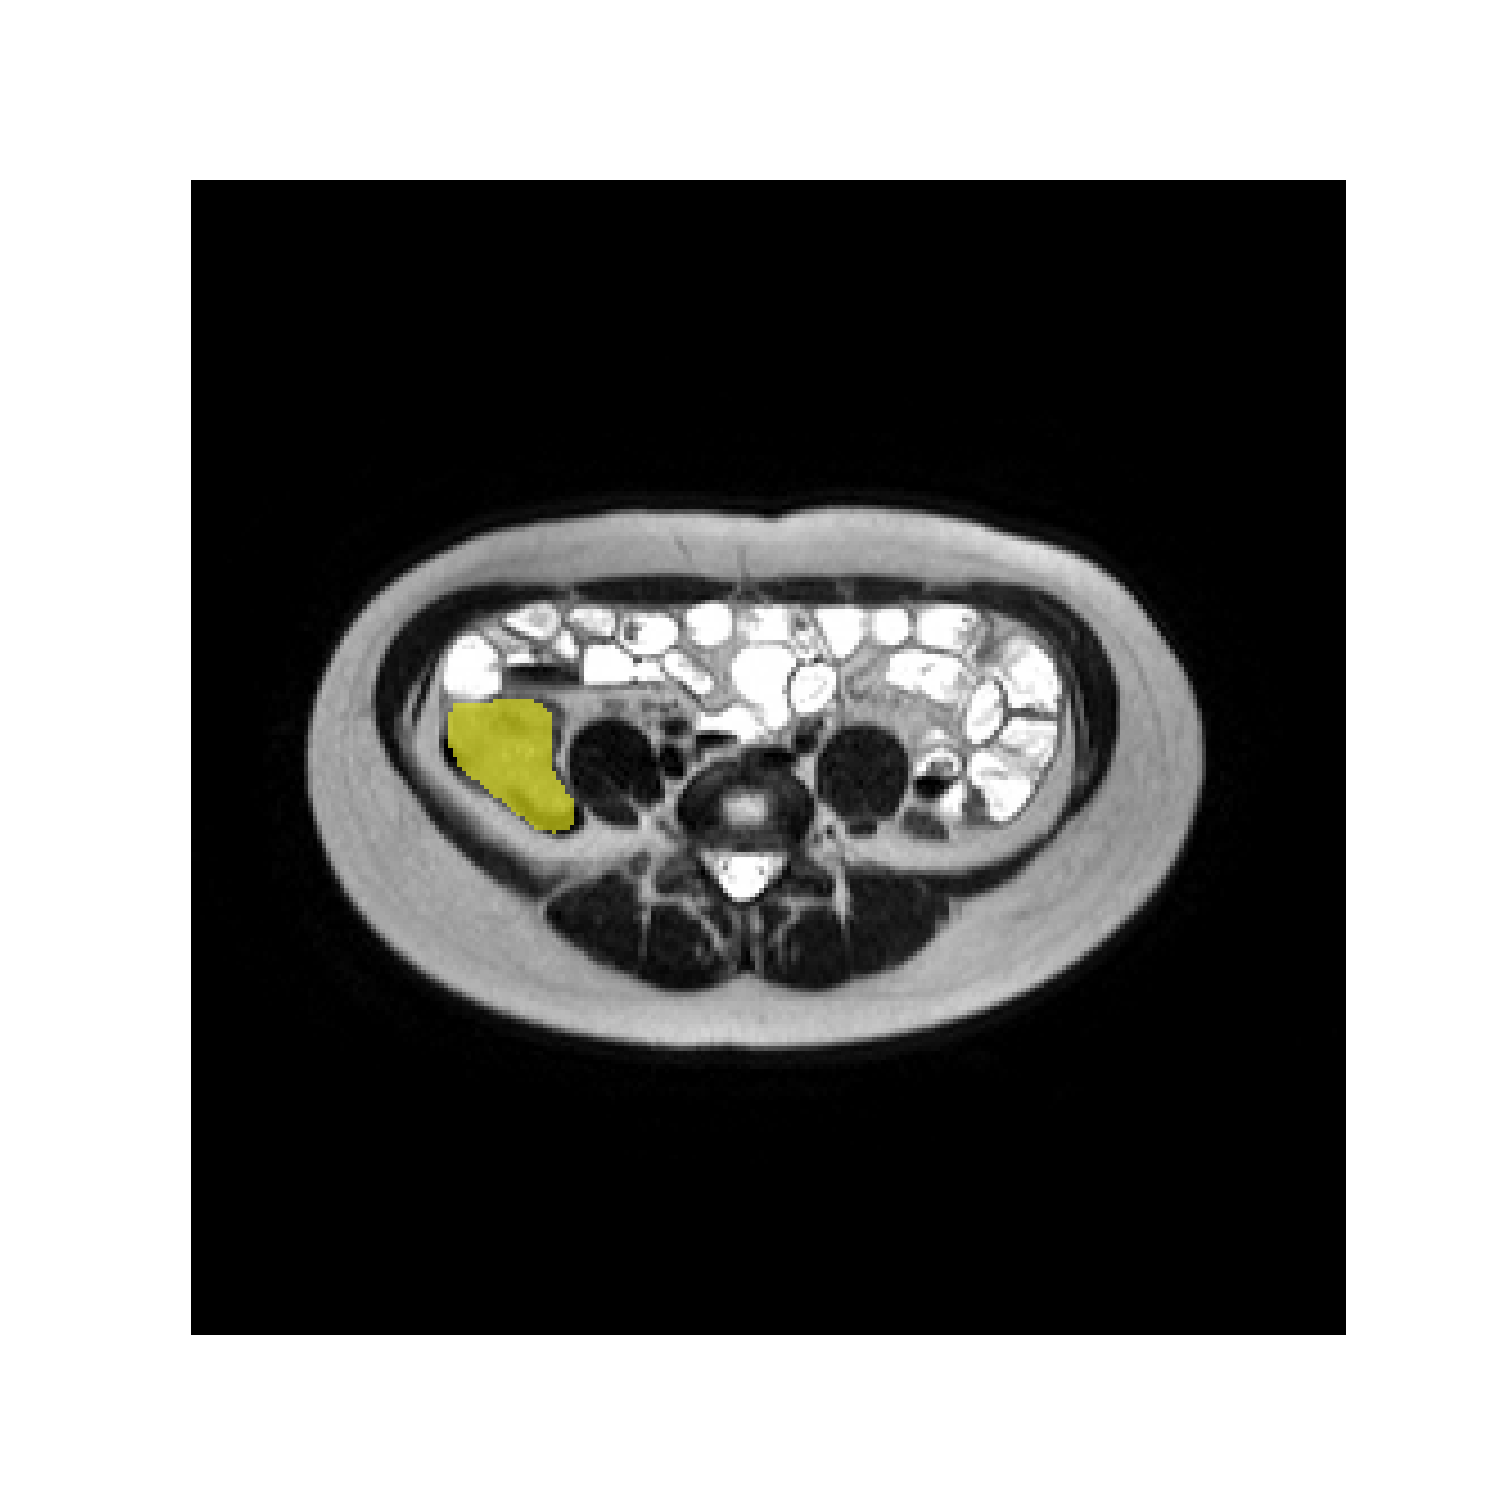
\includegraphics[width=\textwidth]{./figures/seg_medsam.png}
\caption{Our Model Prediction}
\label{fig:medsam-pred}
\end{subfigure}
\caption{Comparative Segmentation Performance Analysis}
\label{fig:comparison-pred}
\end{figure}

This visual analysis highlights the noticeable prevalence of false-positive classifications in the baseline prediction. Conversely, comparing our model and the ground truth reveals a significant alignment, barring minor discrepancies around the boundary contours. These findings visually affirm the advancements we have achieved in the T.I. segmentation, underscoring the superiority of our approach over the prior work.

\subsection{Statistical Evaluation for Establishing Significance}
We conducted an additional t-test, maintaining the parameters specified earlier while assessing the generated weak labels. The table below delineates the decisive outcomes of these t-tests:

\begin{table}[ht]
\centering
\begin{tabular}{c|c|c|c}
Modality & \(t\) statistic & \(p\) value & significance level \\
\hline
Axial & 1.4492 & 0.1853 & 0.05 \\
\hline
Coronal & 1.3816 & 0.1860 & 0.05
\end{tabular}
\end{table}

Though we observed a considerable increase in the mean score and a comparable or even reduced standard deviation, the \(p\) values for both cases surpassed the 0.05 significance threshold. This outcome implies insufficient evidence to invalidate our null hypothesis or substantiate any improvements in the test results. Such contradiction is intriguing, particularly given the apparent disparity and enhancement between the baseline and our proposed approach.

This finding potentially signifies an underpowered study, possibly due to the limited sample size. Even a seemingly substantial disparity in means may not yield statistical significance in such conditions. It might be beneficial to explore alternative statistical measures such as Cohen's d to gauge the magnitude of the improvement more accurately.

\section{Ablation Studies}

Implementing the SAM-based pre-trained model has notably enhanced the quality of the generated weak masks. The training and fine-tuning of the SAM model, including weak label generation, leverage a centerline coordinate file that restricts the bounding box of the T.I. region. In this section, we conduct an ablation study to examine the impact of these centerlines, i.e. T.I. localisation—on the quality of weak labels and to inform potential strategies for subsequent training processes.

We initiated the experiment by refining two SAM models on an identical dataset, one integrated with the bounding box data derived from the centerline and the other devoid of such information. After fine-tuning, both models generated weak masks—one fully informed by the bounding box data and the other operating without it. We applied this methodology on Axial and Coronal images, and the resultant Dice Similarity Coefficient (DSC) was shown in \autoref{tab:ablation-ti}.

\begin{table}[ht]
\centering
\begin{tabular}{c|c|c}
Modality & With localisation & No localisation \\
\hline
Axial & \(0.8084 \pm 0.0695\) & \(0.0802 \pm 0.0115\)\\
\hline
Coronal & \(0.6941 \pm 0.0871\) & \(0.0524 \pm 0.0104\)
\end{tabular}
\caption{Impact of T.I. localisation}
\label{tab:ablation-ti}
\end{table}

These results underscore the diminished performance of the SAM model in the absence of T.I. localisation. This observation (\autoref{fig:4}) finds further validation in the following visual representation of Axial T2 images.

\begin{figure}[htp]
\centering
\begin{subfigure}[b]{0.47\textwidth}
\centering
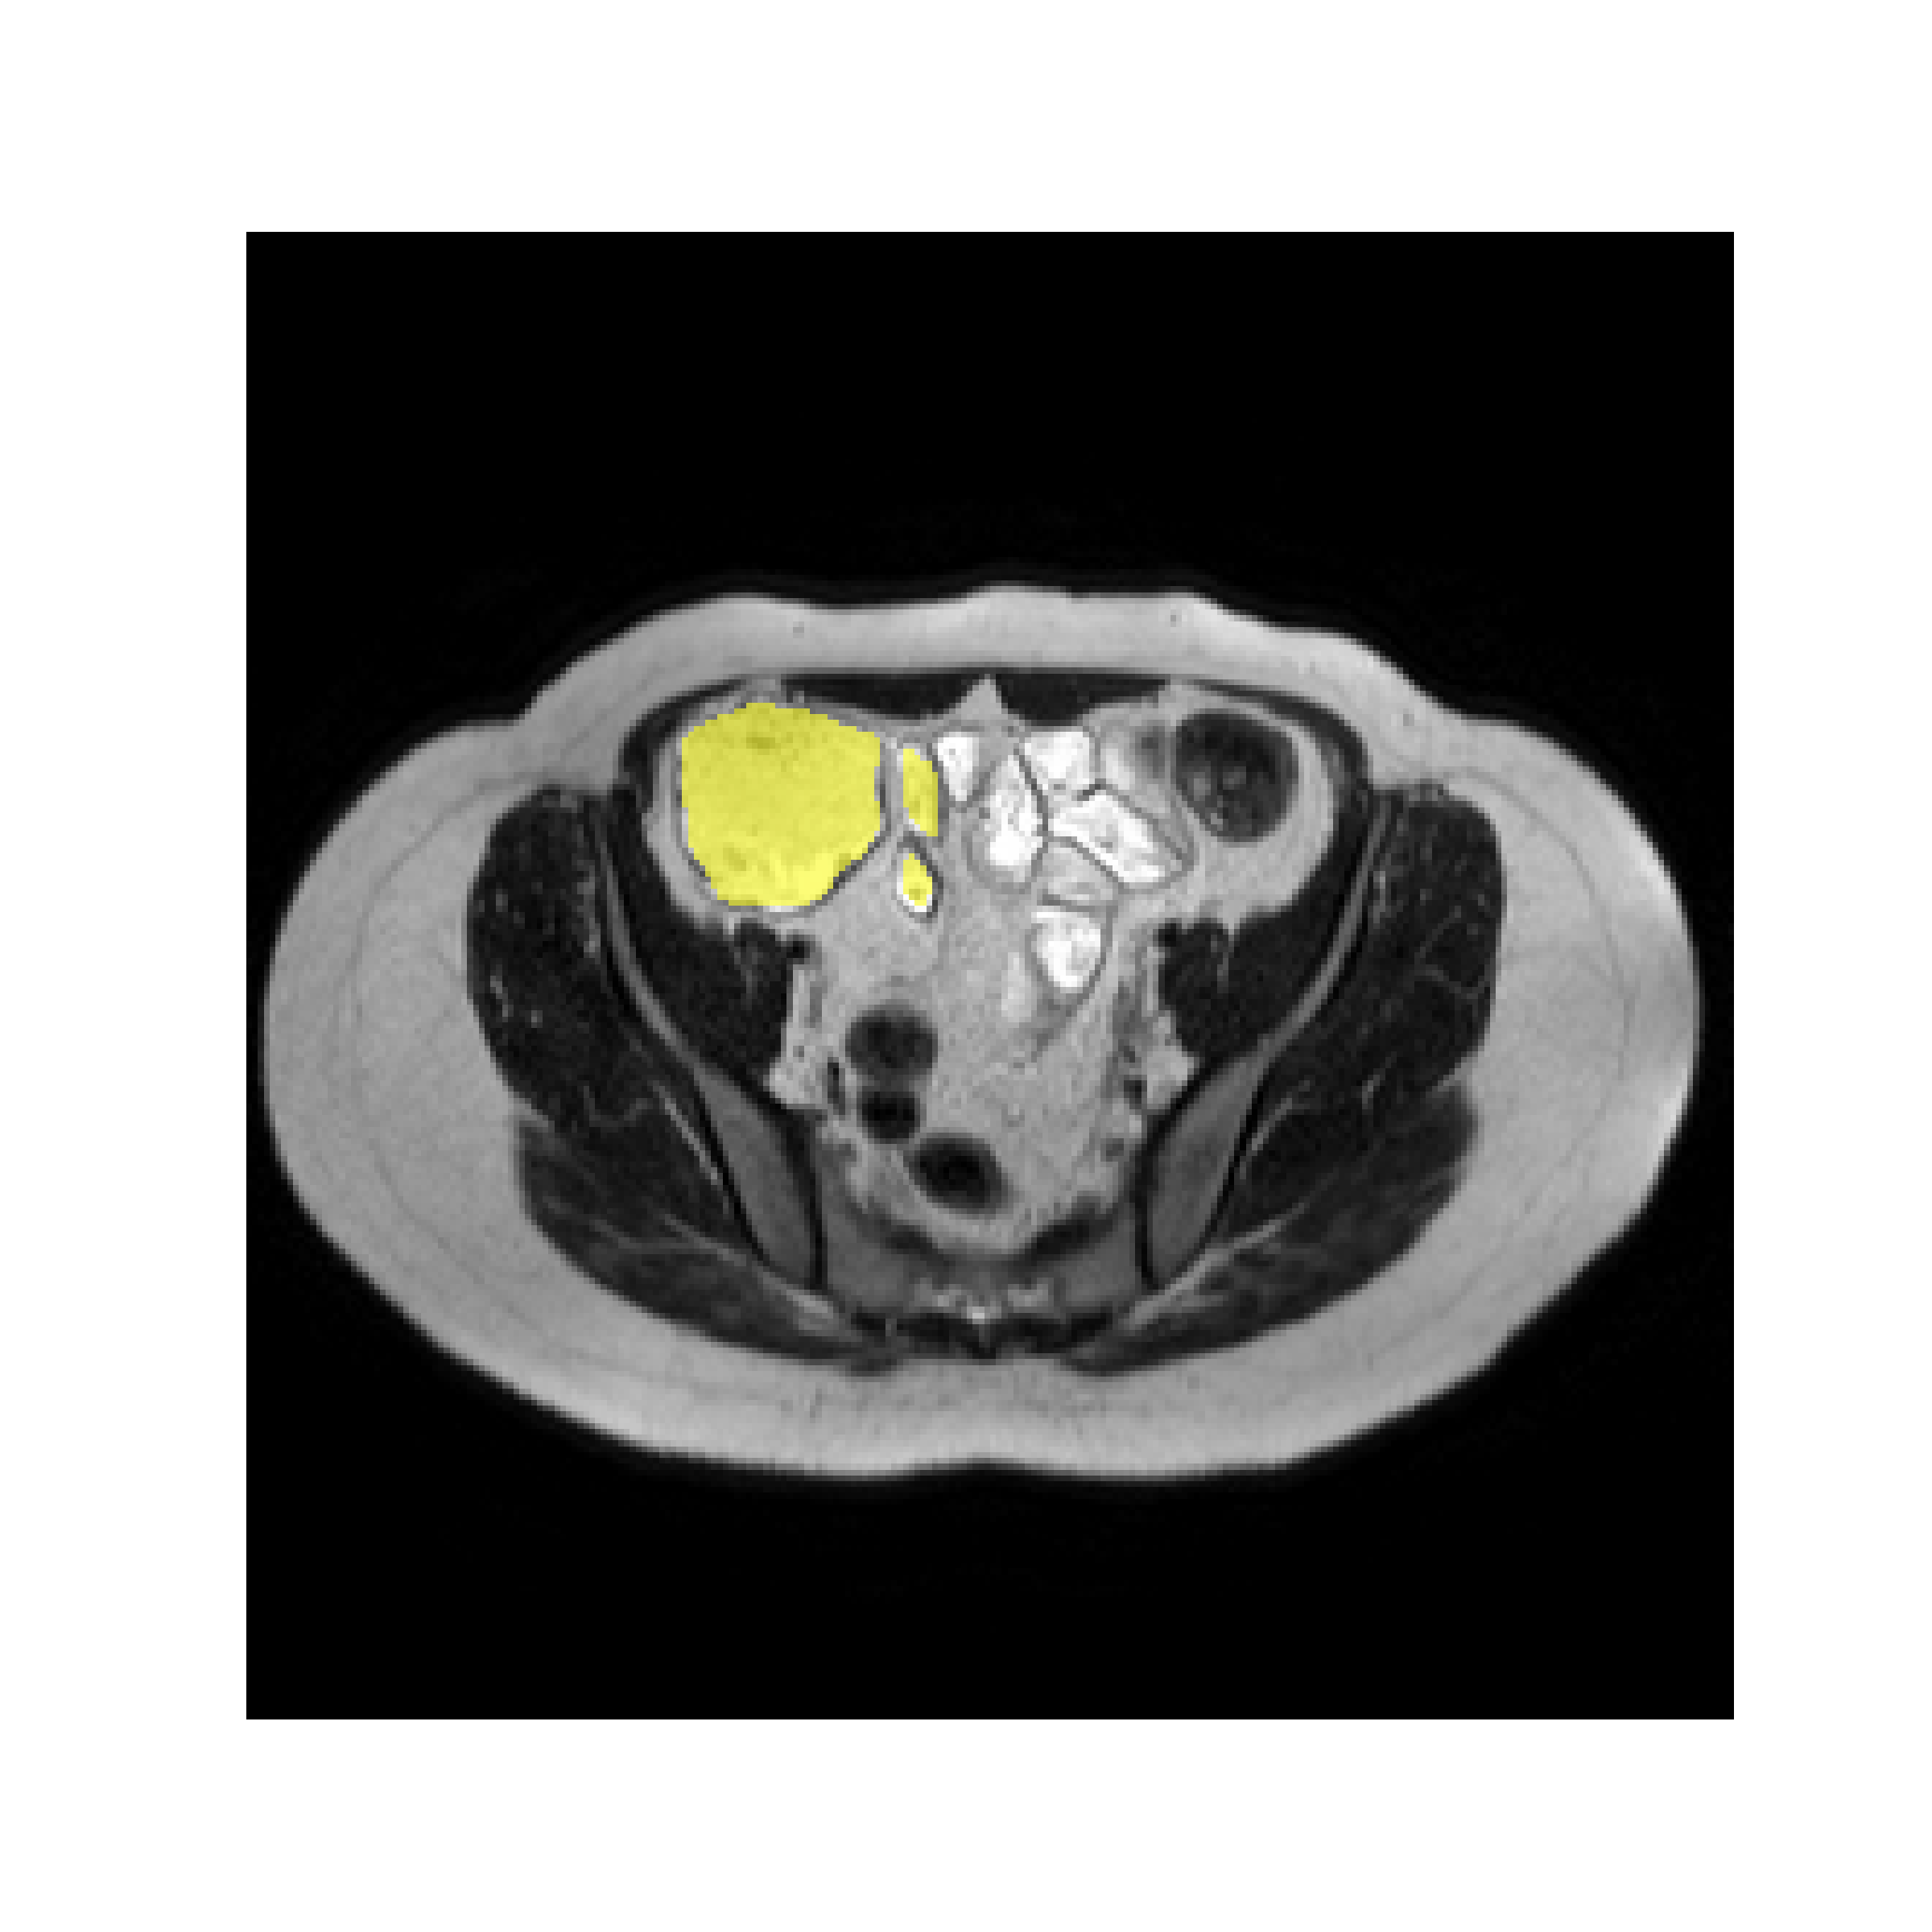
\includegraphics[width=\textwidth]{./figures/ablation_gt.png}
\caption{Ground Truth}
\label{fig:1}
\end{subfigure}
\hfill
\begin{subfigure}[b]{0.47\textwidth}
\centering
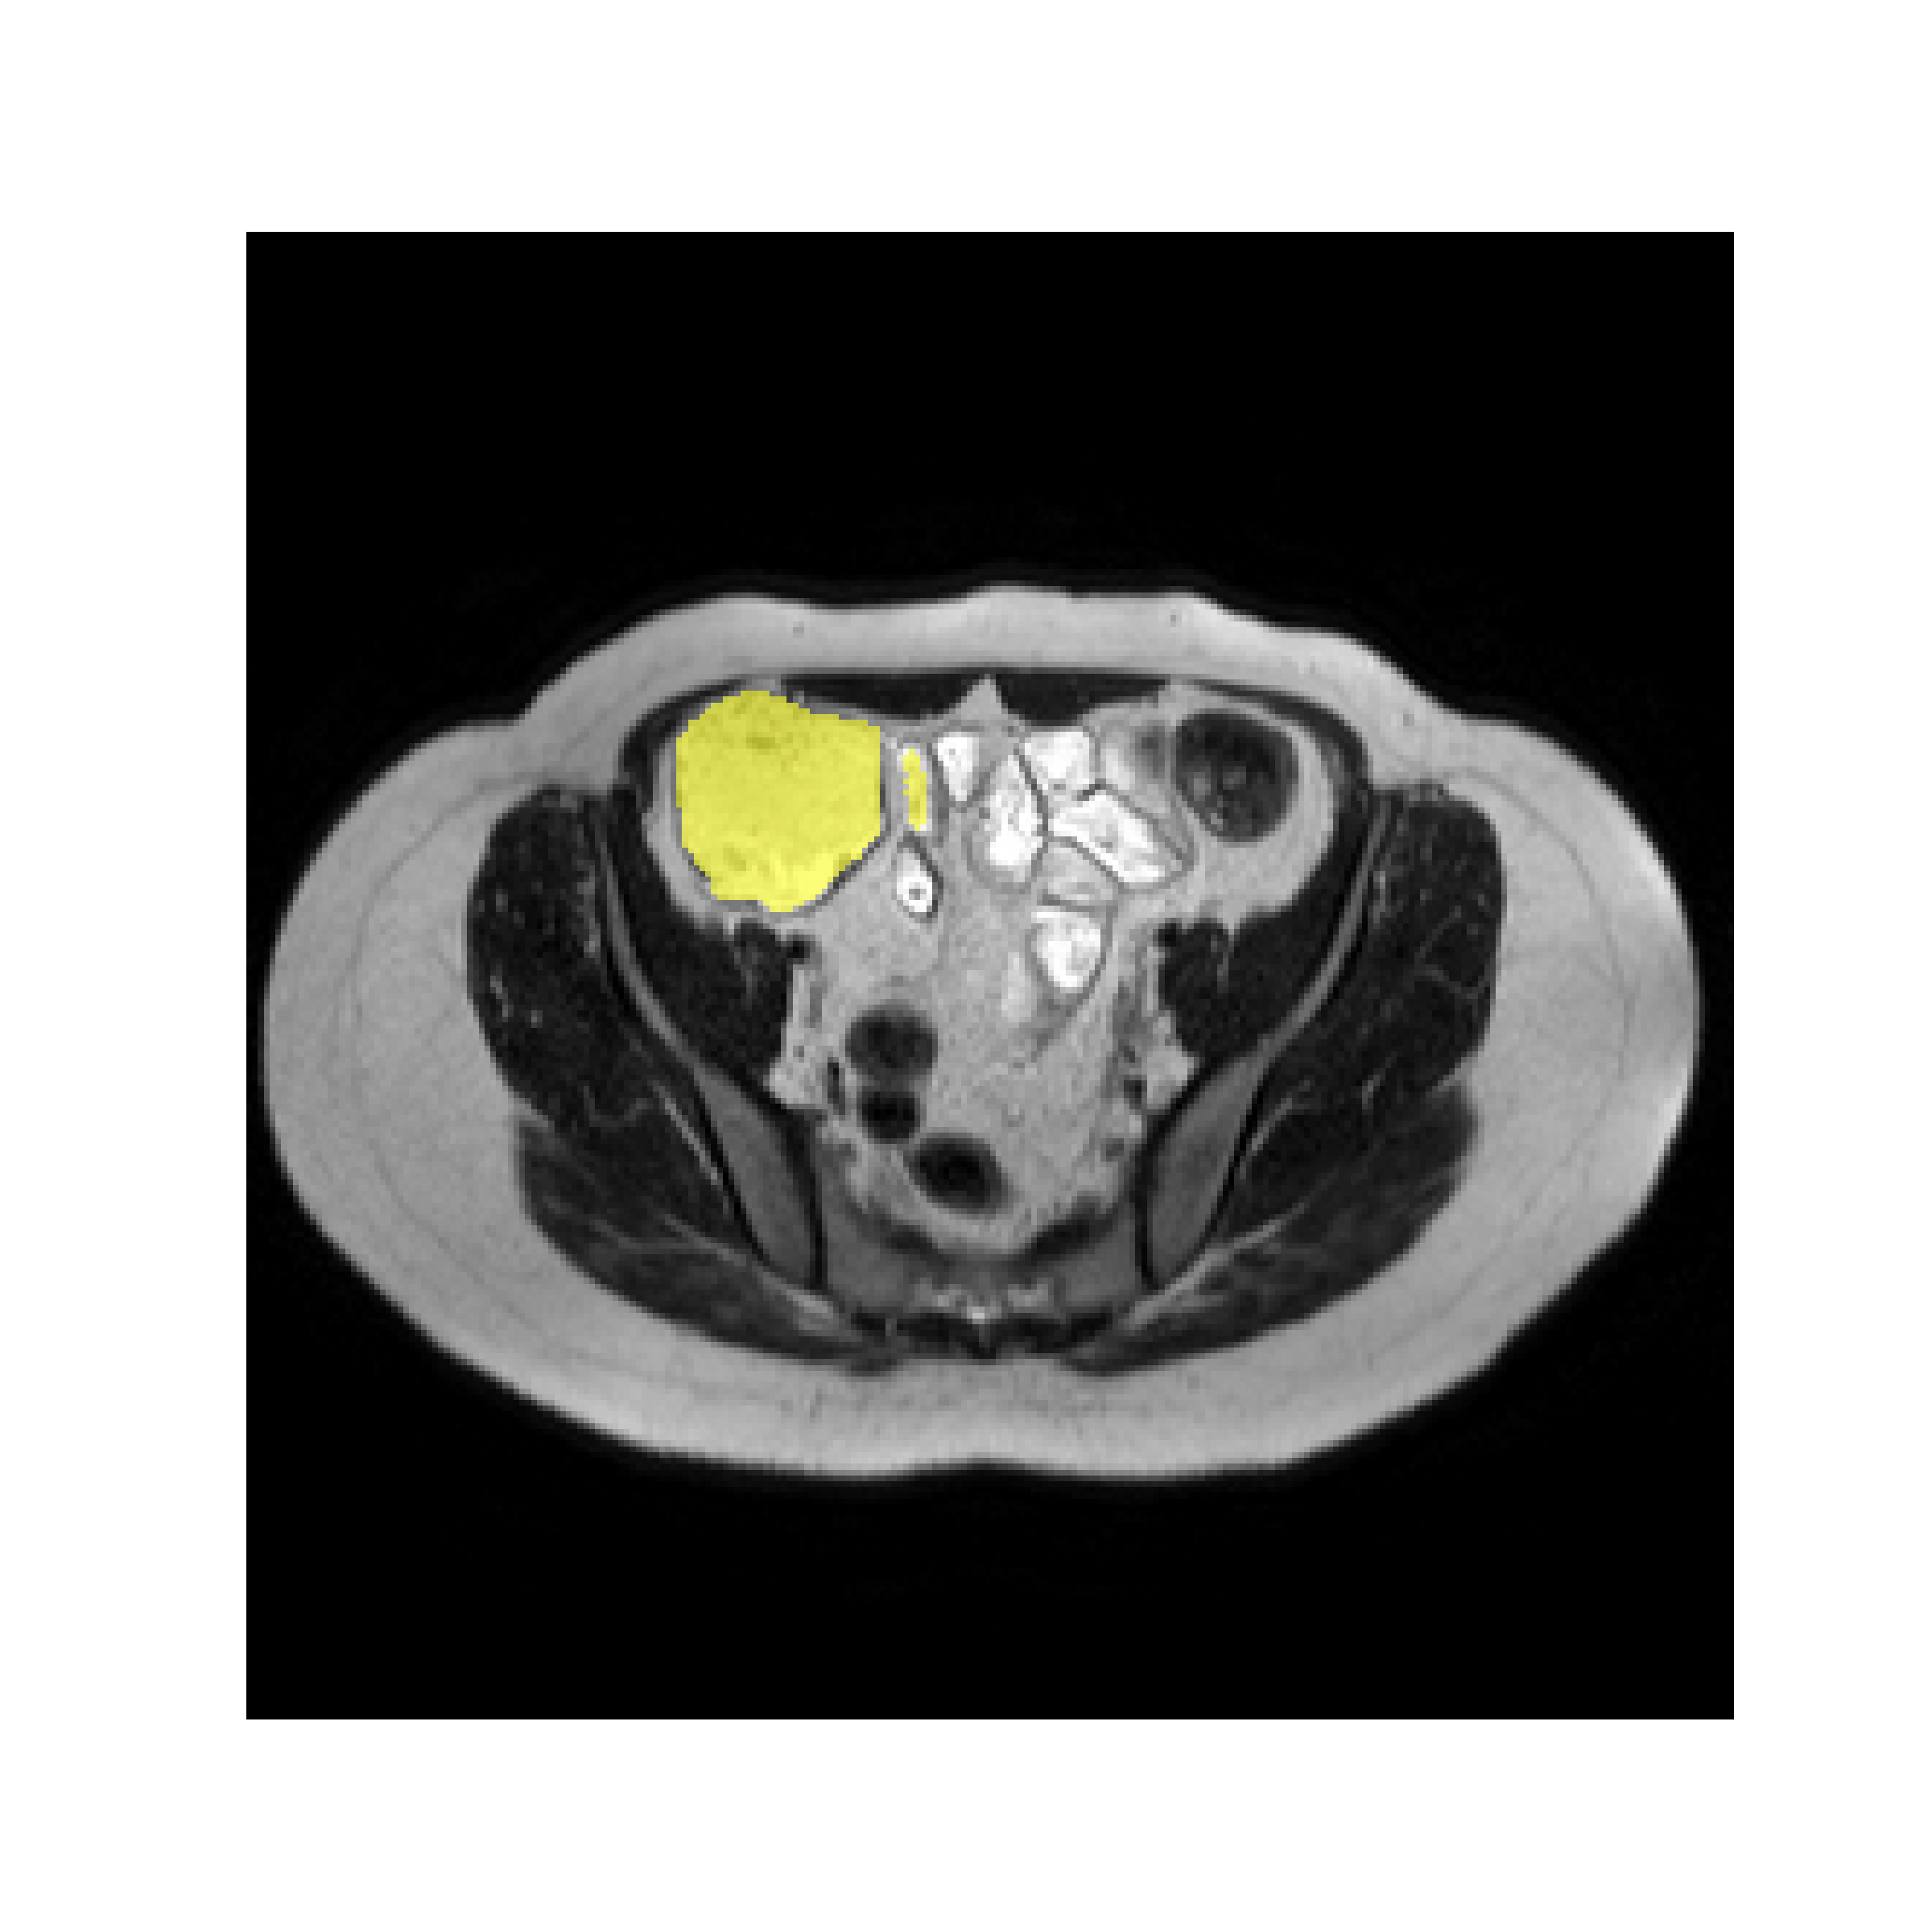
\includegraphics[width=\textwidth]{./figures/ablation_medsam.png}
\caption{Prediction with T.I. localisation}
\label{fig:2}
\end{subfigure}
\hfill
\begin{subfigure}[b]{0.47\textwidth}
\centering
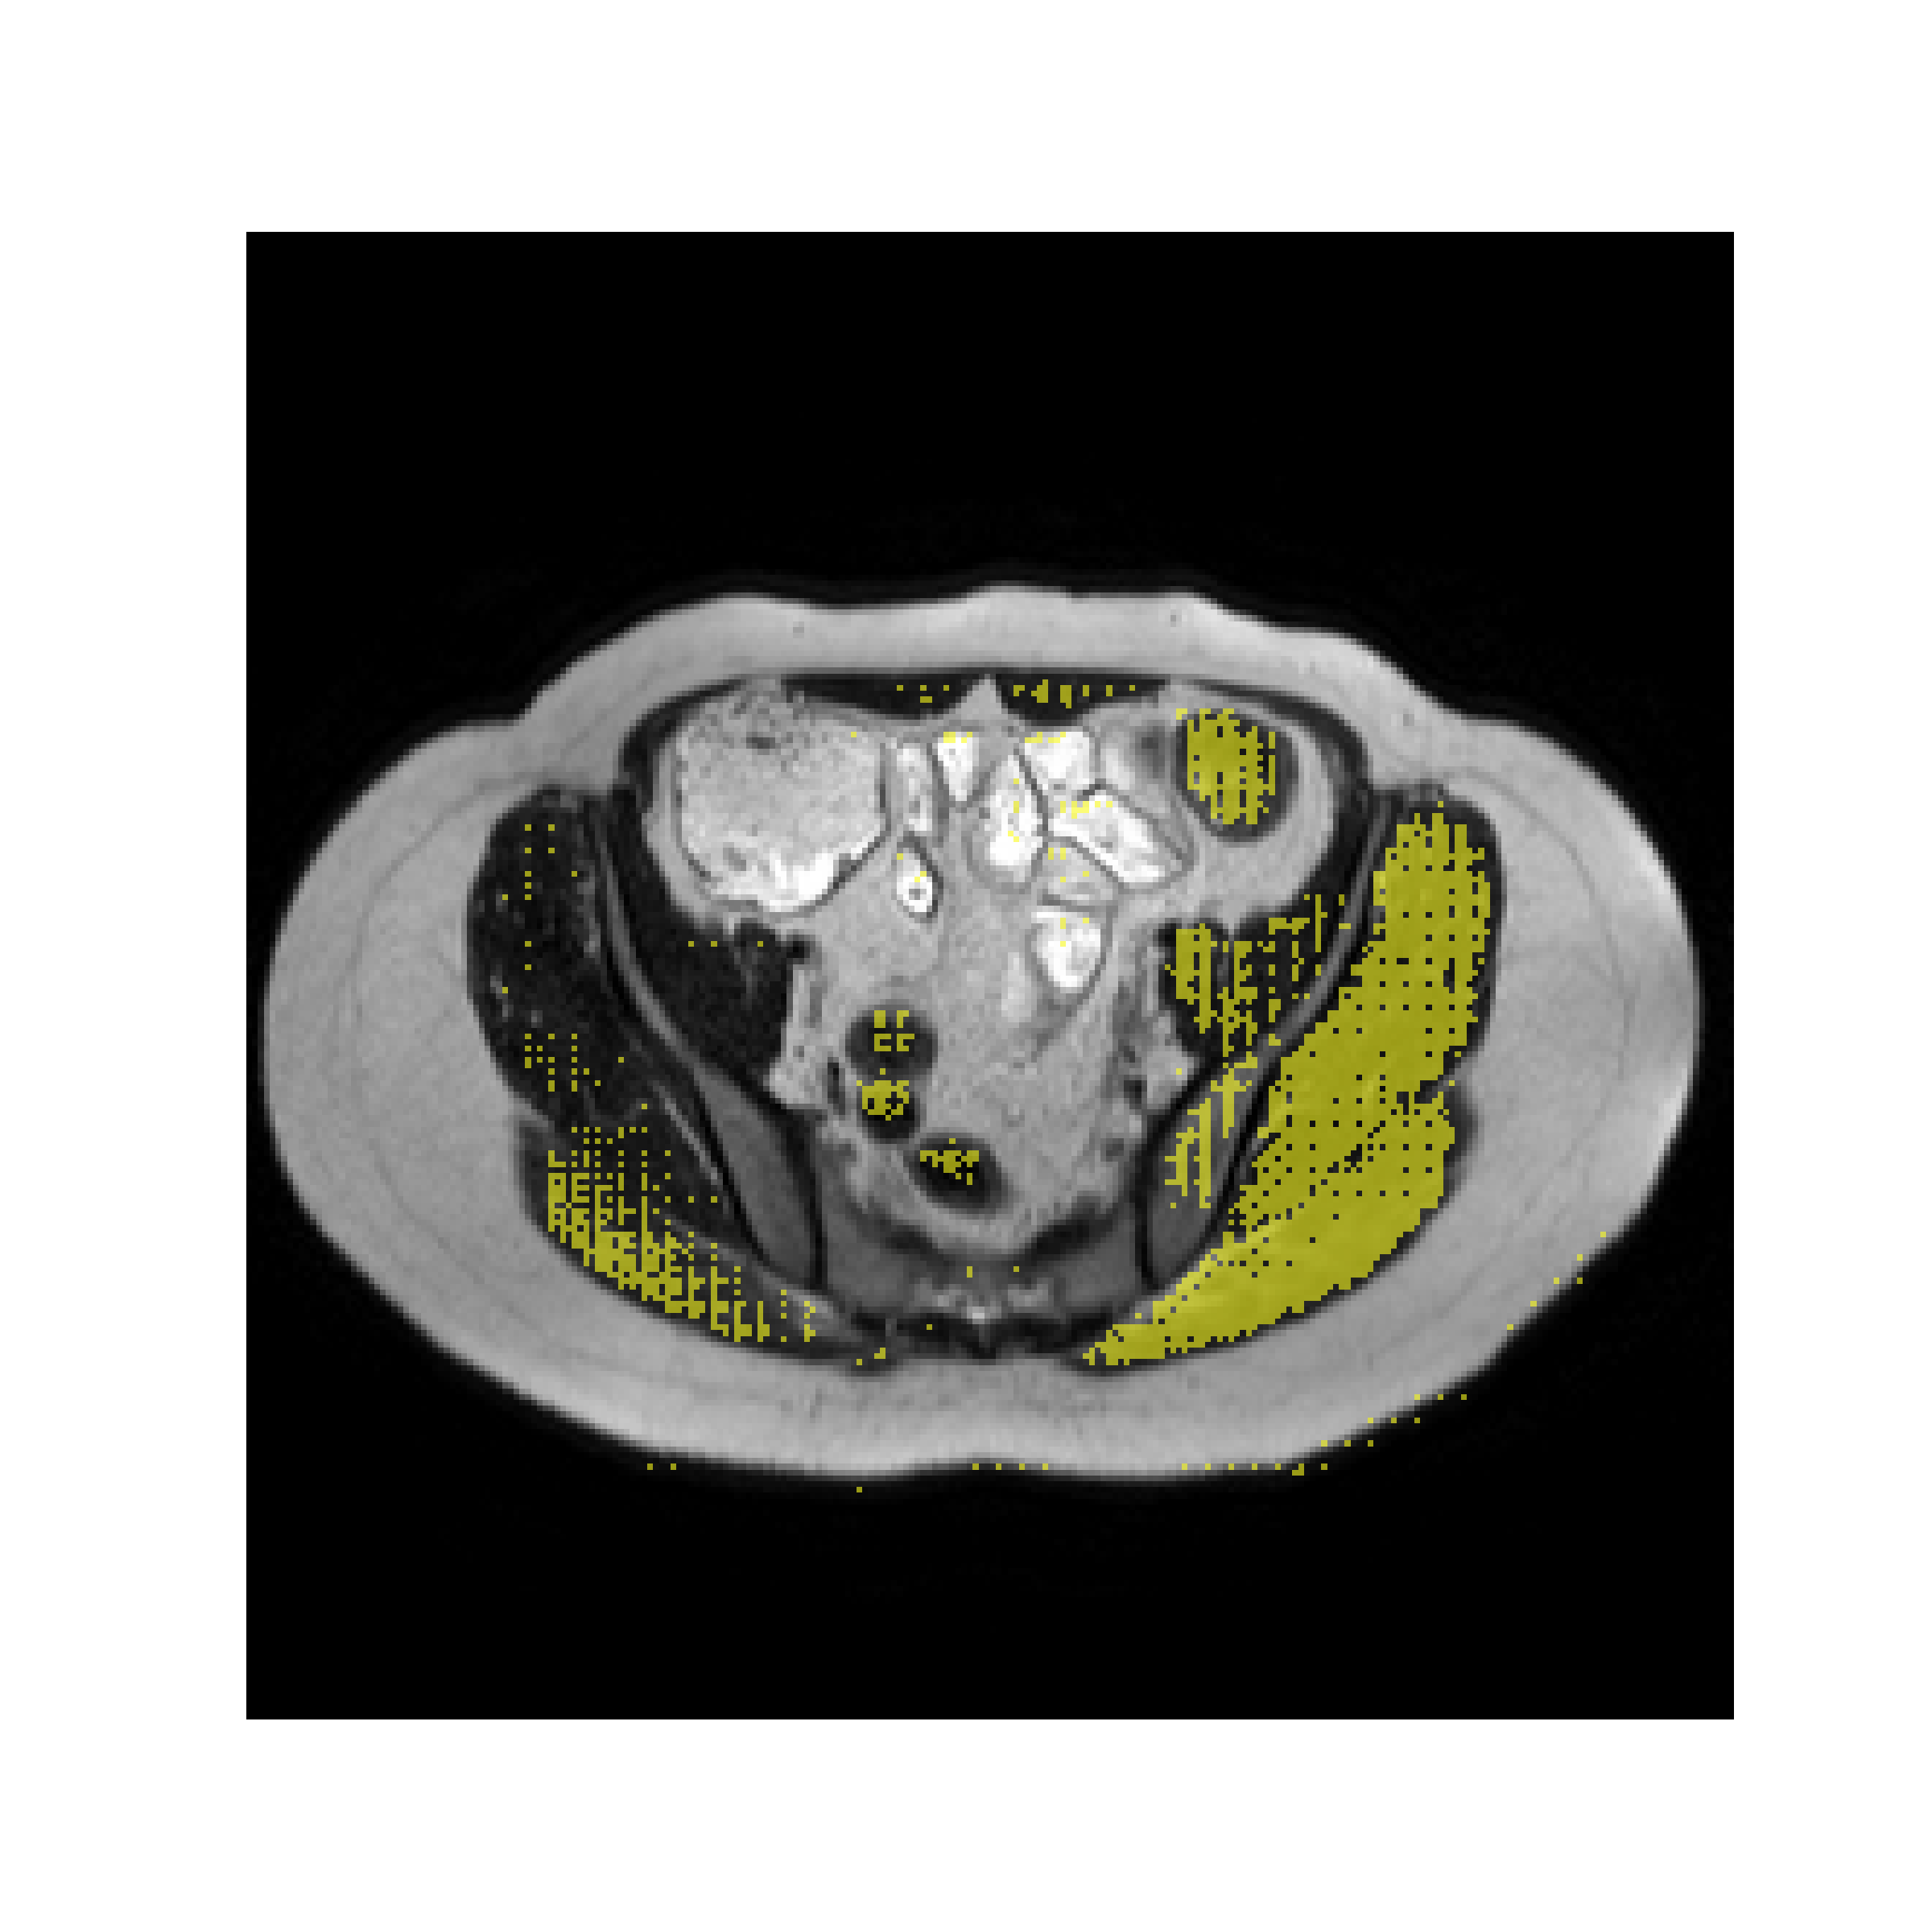
\includegraphics[width=\textwidth]{./figures/ablation_without_loc.png}
\caption{Prediction without T.I. localisation}
\label{fig:3}
\end{subfigure}
\caption{Effect of T.I. Localisation on Mask Generation}
\label{fig:4}
\end{figure}

The visual results presented herein offer compelling evidence underlining the pivotal role of bounding boxes in generating high-quality weak masks or segmentations. This is not a mere enhancement but rather an essential ingredient to optimise the accuracy and quality of predictions. By observing the stark differences in the outcomes, with bounding box localisations leading to significantly superior results, it is clear that this element cannot be overlooked or underestimated in its impact.

In conclusion, our ablation study strongly suggests that localising the T.I. region via bounding box information significantly enhances the quality of weak labels generated by the SAM model. The Dice Similarity Coefficient (DSC) drastically declined when the models operated without centerline localisation, indicating a poor overlap between the predicted and actual results. This finding is consistent across both Axial and Coronal image modalities, as demonstrated by our t-tests and visually reinforced by the comparative images.

Moreover, our findings align with Huang et al. \cite{huang2023segment}, further validating the importance of manual prompts, including points and bounding box information, to enhance the functionality of the SAM model. However, it is worth noting that underperformances in the absence of T.I. localisation do not discount the potential of the SAM model. It only emphasises this specific input's crucial role in enhancing model performance.

As we pivot towards concluding our study and considering future work, it is clear that optimal utilisation of the SAM model for weak mask generation involves carefully considering these localisation factors. This understanding offers a solid foundation for future research efforts, allowing researchers to build upon these results, explore the model's full potential, and improve segmentation quality.